%-------------------------------------------------------------------------
%										PREAMBLE
%-------------------------------------------------------------------------
\documentclass[10pt, aspectratio=169]{beamer}
\usepackage[default, defaultsans, scale=1]{opensans}
\usepackage{appendixnumberbeamer, pgfplots, booktabs, natbib, pgfopts, textpos,ragged2e, epsfig, pstricks, multido, fancyvrb, catchfilebetweentags, pgf, colortbl, cancel, array, pgfplotstable, amsmath}

\usetikzlibrary{calc, positioning, backgrounds, decorations.markings, external, arrows.meta, arrows, shapes, snakes, fit}
\usetikzlibrary{shapes,snakes}
\pgfplotsset{tick label style={font=\small}, label style={font=\small}, legend style={font=\small}, compat= newest}

\setbeameroption{show notes}
%% THEME (I changed the color scheme of the Metropolis theme)
\usetheme[progressbar=frametitle, background=light]{metropolis}

%% GENERAL 
\setbeamertemplate{frametitle continuation}[from second] 
\setbeamertemplate{section in toc}[sections numbered]
\setbeamertemplate{frame numbering}[fraction]
% Justification
\apptocmd{\frame}{}{\justifying}{} 
% Font weight options: l, lc, m, sb, b, eb 
\renewcommand\seriesdefault{l} 
\renewcommand\bfdefault{m} 
\renewcommand\mddefault{l} % this will make equations to pop-up less
% New Section slide format
\AtBeginSection[] 
{
	\begin{frame}
		\frametitle{\secname}
		\tableofcontents[currentsection, hideallsubsections]
	\end{frame}
}

%% Logo on top
% \addtobeamertemplate{frametitle}{}{%
% \begin{textblock*}{100mm}(.97\textwidth,-1.1cm)
% \includegraphics[scale=0.15]{src/UBClogoW}
% \end{textblock*}}

%% Graphs Color Palette 
\definecolor{UBCblue}{RGB}{12, 35, 68} 
\definecolor{UBClblue}{RGB}{0, 85, 183}
\definecolor{UBCgreen}{RGB}{88, 162, 41} 
\definecolor{UBCred}{RGB}{203, 29, 56}
\definecolor{UBCgrey}{RGB}{116, 145, 163}

\definecolor{c3}{RGB}{110, 196, 232}
\definecolor{c4}{RGB}{0, 206, 209}
\definecolor{c5}{RGB}{0, 153, 153}
\definecolor{c6}{RGB}{134, 179, 0}
\definecolor{c8}{RGB}{255, 214, 51}
\definecolor{c9}{RGB}{255, 153, 0}
\definecolor{c10}{RGB}{255, 83, 26}
\definecolor{c12}{RGB}{153, 15, 12} 



%--------------------------------------------------------------------------------------
%										TITLE PAGE SETUP
%--------------------------------------------------------------------------------------

\title[Git 4 Econ]{Git para economistas} 
\subtitle{Introducción a sistemas de control de versión}
\author{Nicolas Franz-Pattillo}
\institute[VSE]{University of British Columbia}
\date{\today} 

%--------------------------------------------------------------------------------------
%										BEGIN DOCUMENT
%--------------------------------------------------------------------------------------

\begin{document}


%--------------------------------------------------------------------------------------
%										 TITLE FRAME
%--------------------------------------------------------------------------------------
\begin{frame}
	\titlepage
\end{frame}

%--------------------------------------------------------------------------------------
%										 PRESENTATION SLIDES
%--------------------------------------------------------------------------------------

%% TABLE OF CONTENTS
\begin{frame}[allowframebreaks,b]{Table of contents}
	\tableofcontents[hideallsubsections]
\end{frame}

%--------------------------------------------------------------------------------------
%										SECCION: Introduction
%--------------------------------------------------------------------------------------
\section{Introducción}

\begin{frame}{\secname}
	
	\begin{itemize}
		\onslide<1->{
		\item Hoy en día no es raro que los proyectos contengan mas de un archivo.
		\begin{itemize}
			\vfill \item Texto
			\vfill \item Datos y gráficos
			\vfill \item Programas: *.do, *.m, *.prg, etc.  
		\end{itemize}
		}
		\onslide<2->{
		\vfill \item Tampoco es raro que tengan varios co-autores.
		}
	\end{itemize}
	\begin{columns}[onlytextwidth]
		\column{0.4\textwidth}
		\onslide<3->{
		\begin{alertblock}{Problema}
			Cómo hacemos avanzar el proyecto de forma ordenada?
		\end{alertblock}	  
		}
		\onslide<4->{
		\column{0.1\textwidth}
		\centering
		% \vspace{1cm}
		$\implies$
		\column{0.4\textwidth}
		\begin{block}{Solución$^*$}
			Coordinando una forma de hacer los cambios
		\end{block}
		}
	\end{columns}
\end{frame}


\begin{frame}[<+->]{Qué es un sistema de control de versión?}
	\begin{figure}[H]
		\centering
		\caption{PhD Comics \# 1531}
		
\includegraphics[width=0.3\textwidth]{src/images/finalVersion.png}
	\end{figure}
\end{frame}


\begin{frame}[<+->]{Qué es un sistema de control de versión?}
	\begin{figure}[H]
		\centering
		\caption{Control de versión ``naive''}
		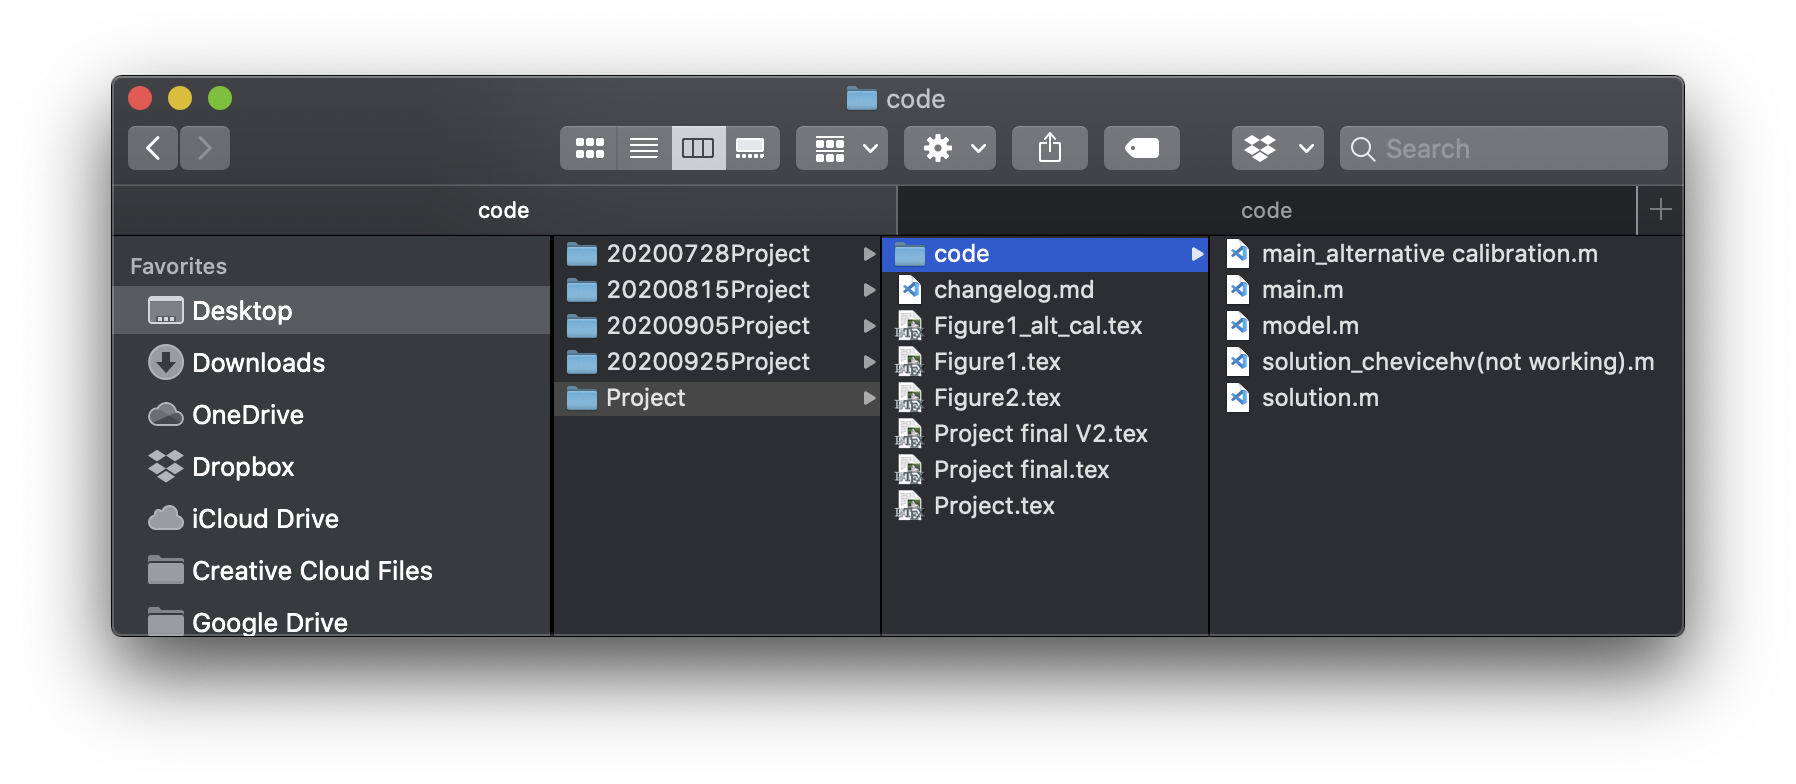
\includegraphics[width=0.8\textwidth]{src/images/projectBeforeGit.png}
	\end{figure}
	\pause
	\begin{itemize}
		\vfill \item Los programadores han tenido este problema por décadas.
		\vfill \item Las soluciones (\emph{software}) han ido evolucionando con el tiempo. En general se les conoce como \textbf{sistemas de control de versión}
		\vfill \item La mayoría de ellos presenta al usuario la versión que se quiere revisar y deja el resto fuera de la vista.
	\end{itemize}
\end{frame}

\begin{frame}[<+->]{Repo, commit, working copy ... me no english!}
	Los \emph{softwares} de control de versión comparten una terminología común \textcolor{UBCgrey}{(al igual que muchos lenguajes de programación comparten el condicional \emph{if... then... else} y los bucles \emph{for} o \emph{while} )}
	\begin{enumerate}
		\vfill \item \textbf{Commit}: Fotografía del proyecto en un momento del tiempo determinado
		\vfill \item \textbf{Repository}: (``Repo'') Proyecto completo, incluyendo su historia.
		\vfill \item \textbf{Working copy}: Versión del proyecto en la cual se está trabajando.
	\end{enumerate}
\end{frame}

\begin{frame}{Tipos de control de versión}
	\begin{enumerate}
		\item Locales
		\vfill \item Distribuidos
		\vfill \item No distribuidos
	\end{enumerate}
\end{frame}

\begin{frame}{Tipos de control de versión}
	\begin{columns}[T, onlytextwidth]
		\column{0.5\textwidth}
		\begin{figure}
			\centering
			\caption{Sistema Distribuido}
			\ExecuteMetaData[src/texGraphs/distributedDiagram.tex]{tikzPic}
		\end{figure}
		\column{0.5\textwidth}
		\begin{figure}
			\centering
			\caption{Sistema No Distribuido}
			\ExecuteMetaData[src/texGraphs/nonDistributedDiagram.tex]{tikzPic}
		\end{figure}
	\end{columns}
\end{frame}

\begin{frame}[standout]{Tipos de control de versión}
	Preguntas?
\end{frame}
%--------------------------------------------------------------------------------------
%										SECCION: GIT
%--------------------------------------------------------------------------------------
\section{Git}
\subsection{Qué es Git?}

\begin{frame}[<+->]{\subsecname}
	\begin{itemize}
		\item Git es un sistema distribuido de control de versión. El más utilizado en el mundo.
		\vfill \item El \emph{software} de Git se instala ``localmente''. \textcolor{UBCgrey}{Para empezar a utilizar Git no es necesario un servidor. No obstante, este último mejora la colaboración significativamente. }
		\vfill \item \alert{Git no es lo mismo que GitHub!} \textcolor{UBCgrey}{GitHub es una red social que utiliza la arquitectura Git como base. Otros ejemplos son GitLab y BitBucket.}
	\end{itemize}
\end{frame}

\subsection{Cómo se usa Git?}
\begin{frame}{\subsecname}
	\begin{itemize}
		\item Git se usa a través de la linea de comando.
		\begin{itemize} 
			\item \textcolor{UBCgrey}{MacOS: Terminal} 
			\item \textcolor{UBCgrey}{Windows: Command Prompt o PowerShell}
		\end{itemize}
		\begin{figure}
			\centering
			\caption{iTerm terminal en MacOs}
			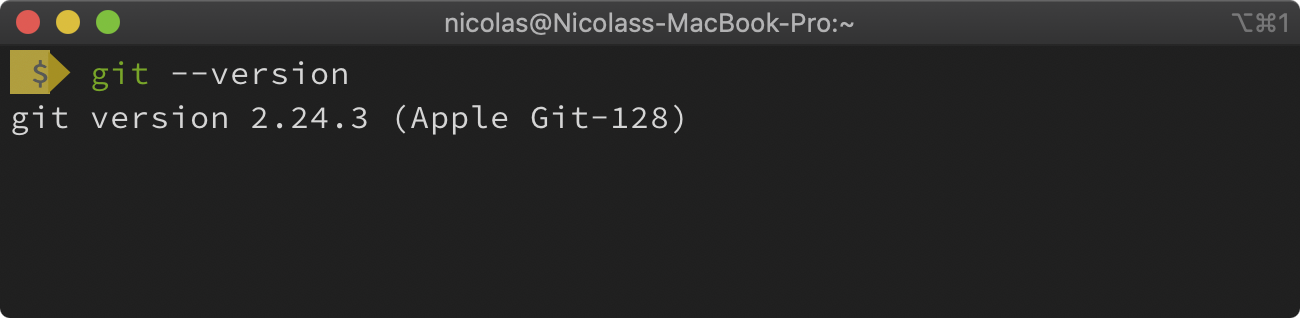
\includegraphics[width=0.5\textwidth]{src/images/iTerm-gitVersion.png}
		\end{figure}
		\vfill \item Git es parte de la distribución de otros \emph{softwares}, por lo que puede que ya lo tengas instalado. \textcolor{UBCgrey}{(e.g., Python-Anaconda, o command line tools de MacOs, \href{https://www.mathworks.com/help/matlab/matlab_prog/set-up-git-source-control.html}{Matlab 2020b}).}
	\end{itemize}
\end{frame}

\begin{frame}{\subsecname}
	\begin{itemize}
		\item Hay muchas otras interfaces de usuario gráficas (GUI) que lo hacen mas amigable 
	\end{itemize}
	\begin{figure}
		\centering
		\caption{Integración Git, VS Code}
		\vspace{-0.5cm}
		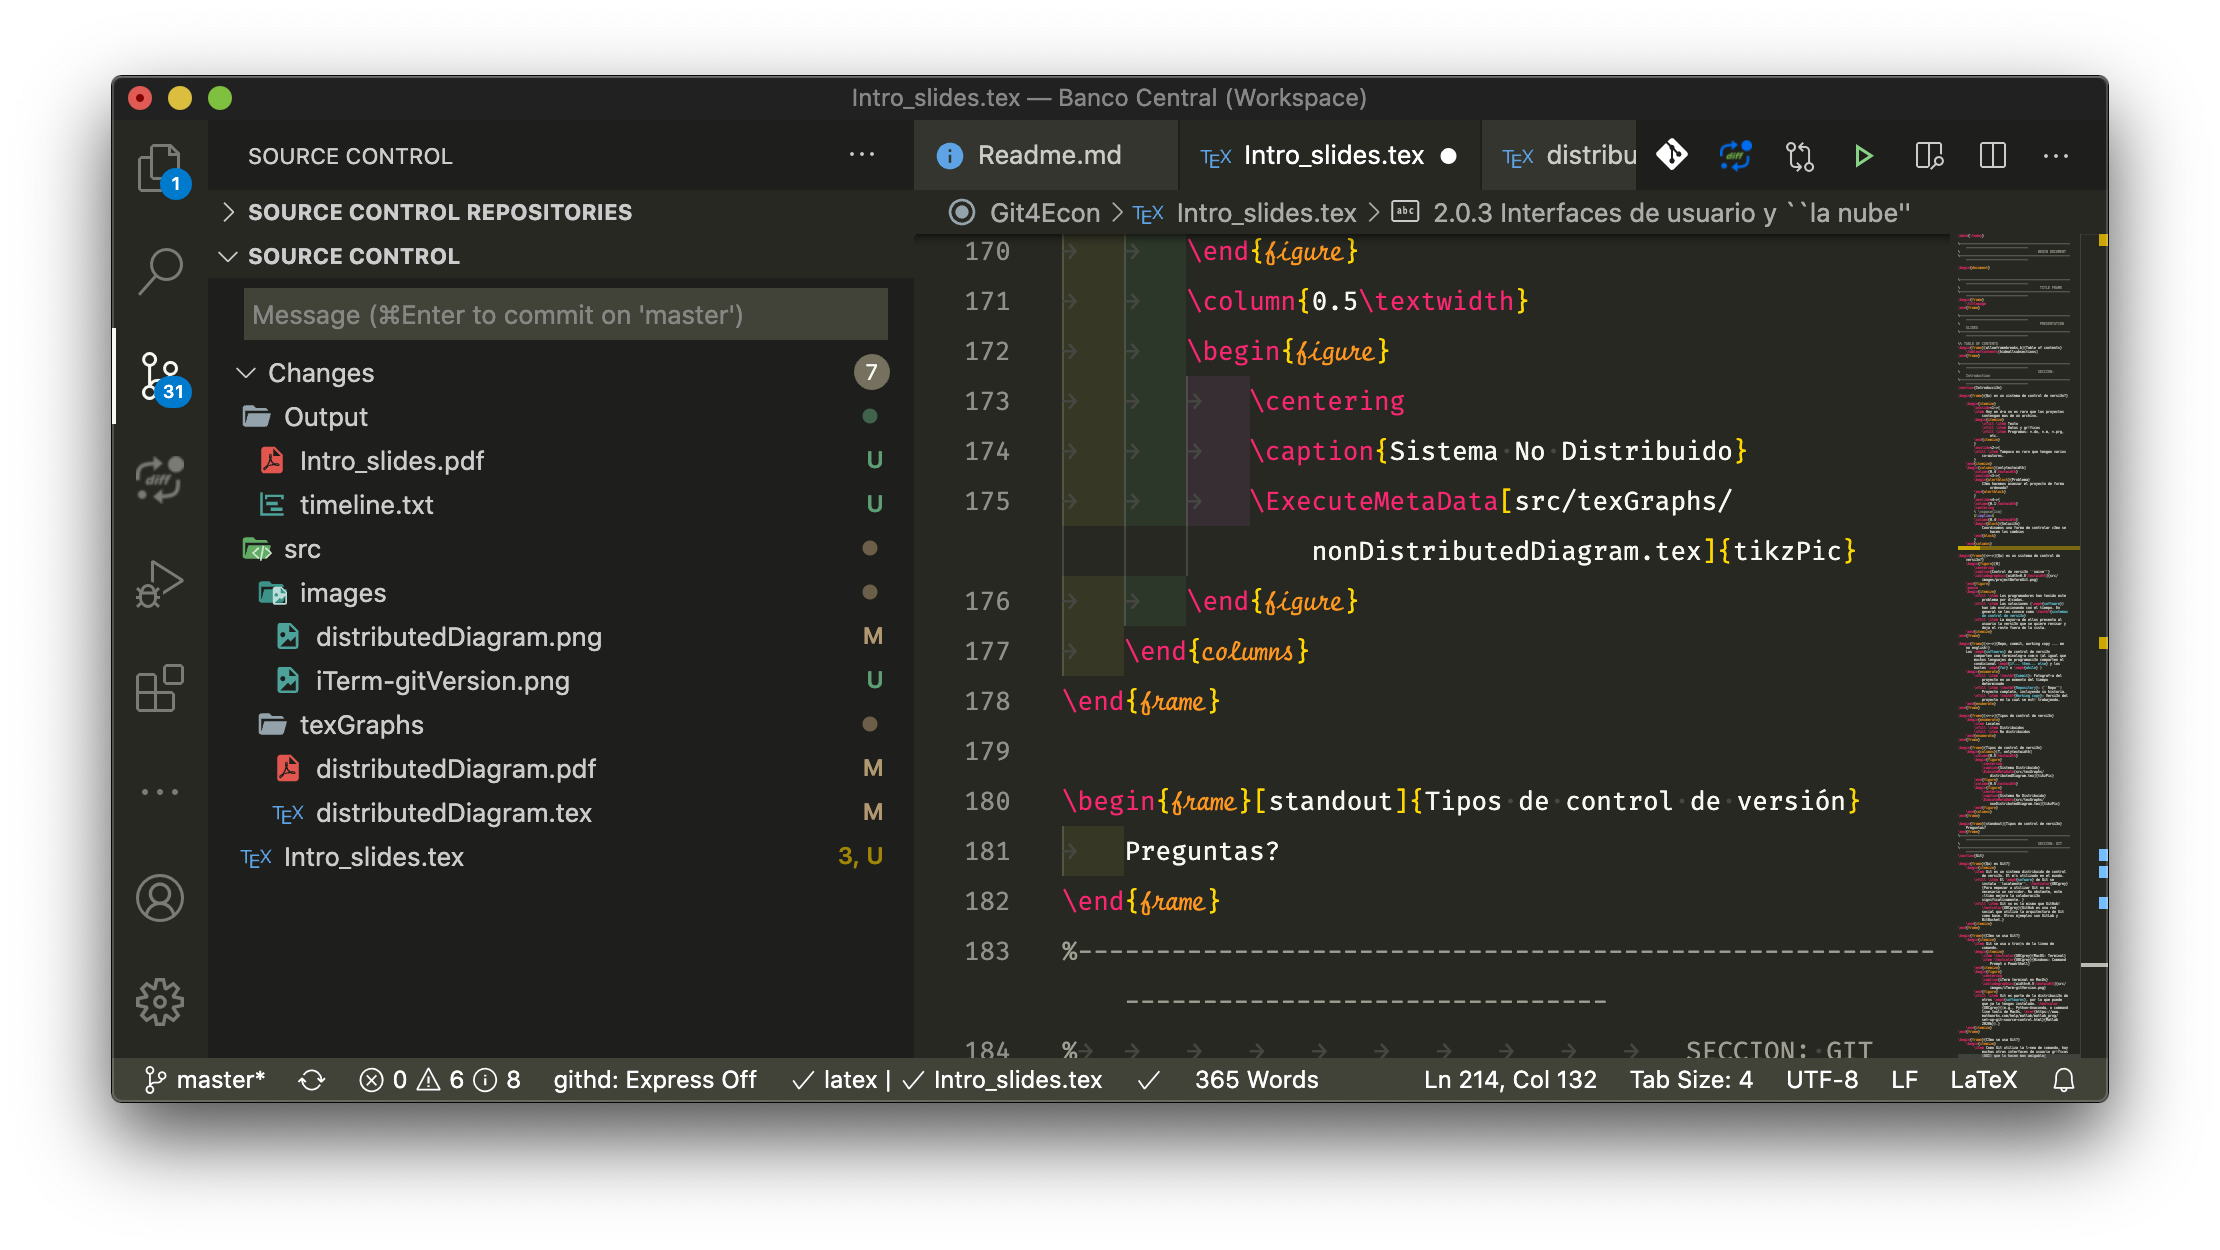
\includegraphics[width=0.8\textwidth]{src/images/VSCode.png}
	\end{figure}
\end{frame}

\begin{frame}{\subsecname}
	\begin{itemize}
		\item Hay muchas otras interfaces de usuario gráficas (GUI) que lo hacen mas amigable
	\end{itemize}
	\begin{figure}
		\centering
		\caption{Integración Git, Matlab}
		\vspace{-0.6cm}
		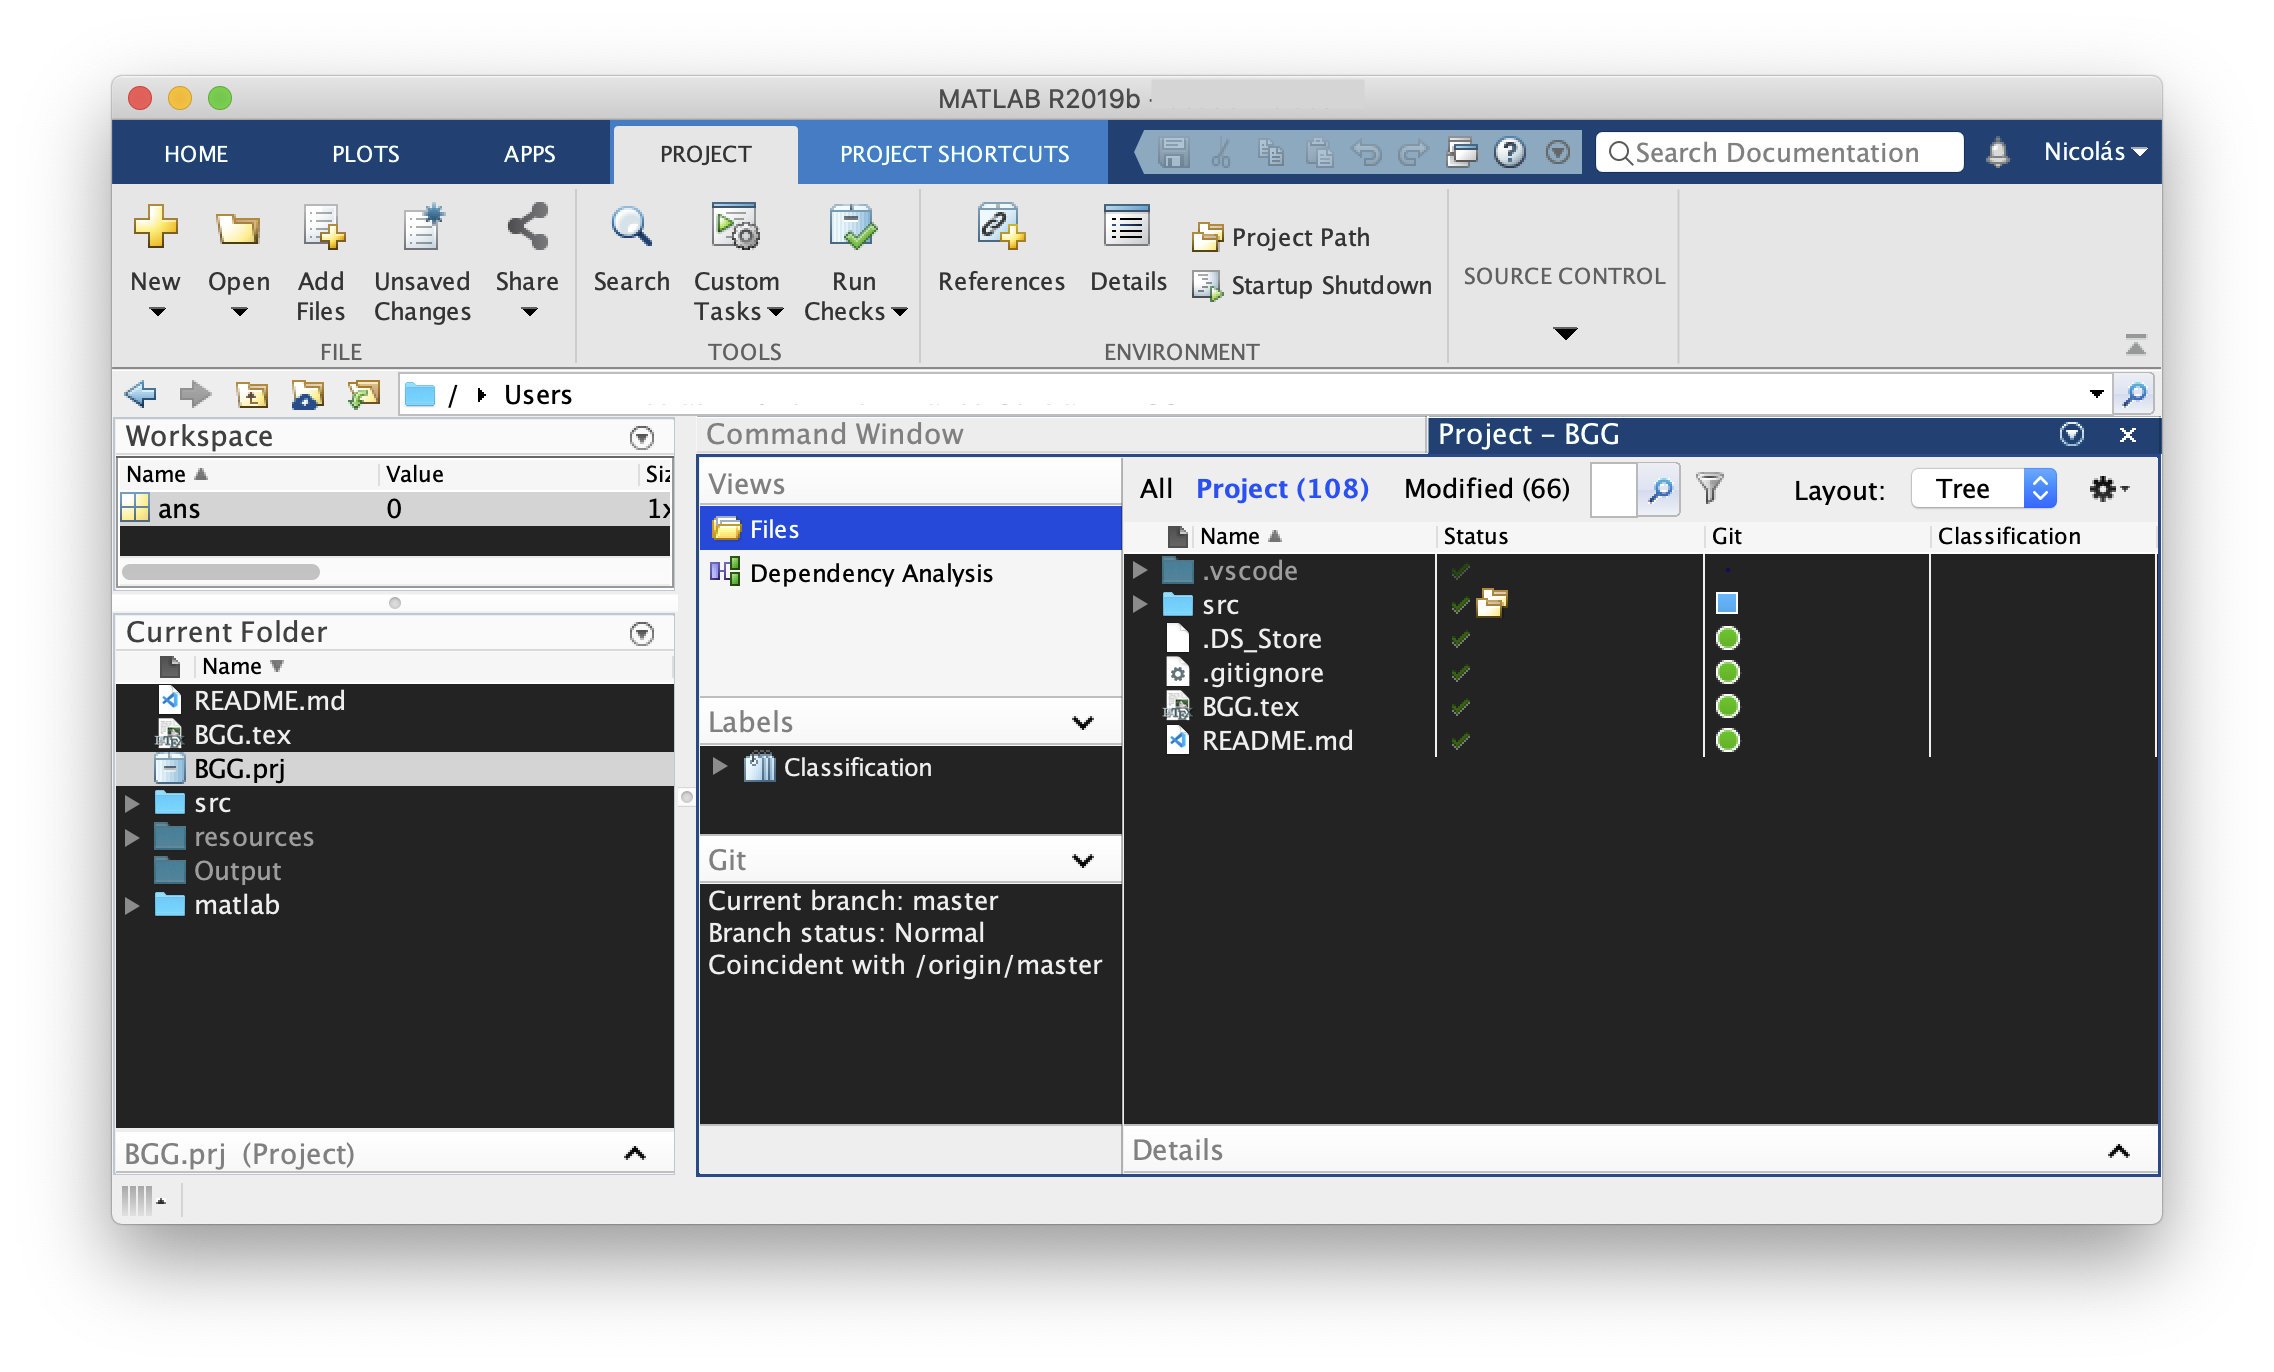
\includegraphics[width=0.7\textwidth]{src/images/matlab.png}
	\end{figure}
\end{frame}

\begin{frame}[<+->]{\subsecname}
	\begin{itemize}
		\item La forma estándar de aprender Git es a través de la línea de comando.
		\vfill \item Esto no quiere decir que el usuario lo use a través de ella, pero le da uniformidad al proceso \textcolor{UBCgrey}{(Las GUI pueden tener formas diversas de implementar Git y aprenderlas es difícil si no se entiende el objetivo. Es como querer aprender MS excel sin saber matemáticas)}
		\vfill \item Con el tiempo, el uso y la terminología Git se vuelve natural... \onslide<+->{trust me!}
	\end{itemize}
\end{frame}

\begin{frame}[standout]{\secname}
	Preguntas?
\end{frame}

\subsection{Trabajo no lineal}
\begin{frame}[<+->]{\subsecname}  
	\begin{itemize}
		\item Una de las grandes ventajas de Git es que simplifica el uso de ``ramas'' o estructuras no lineales 
	\end{itemize}
	\begin{figure}[H]
		\centering
		\caption{Árbol Git, ejemplo}
		\ExecuteMetaData[src/texGraphs/branchesExample.tex]{tikzPic}
	\end{figure}
\end{frame}

\begin{frame}[<+->]{\subsecname}  
	\begin{exampleblock}{Ejemplo A: el uso de ramas para experimentar}
		\begin{enumerate}
			\item Empezamos a trabajar en un nuevo modelo estructural.
			\item Inicializamos el repositorio git y creamos algunos códigos: solución y parametros base.
			\item Hacemos el primer \emph{commit} con ambos archivos para luego empezar a escribir un documento en \LaTeX
			\item Hacemos un segundo \emph{commit} incluyendo el texto anterior.
			\item Creamos la rama ``Opcionales'' para explorar otros parámetros.
			\item Hay un error en la solución del modelo! Volvemos a la rama ``master'' para solucionarlo.
			\item Volvemos a explorar en ``Opcionales'' (actualizando la solución) y llevamos los resultados de ``Opcionales'' a ``Master''
		\end{enumerate}
	\end{exampleblock}
\end{frame}

\begin{frame}[<+->]{Ejemplo A}  
	\begin{exampleblock}{Cómo inicializar un repositorio}
			\centering
			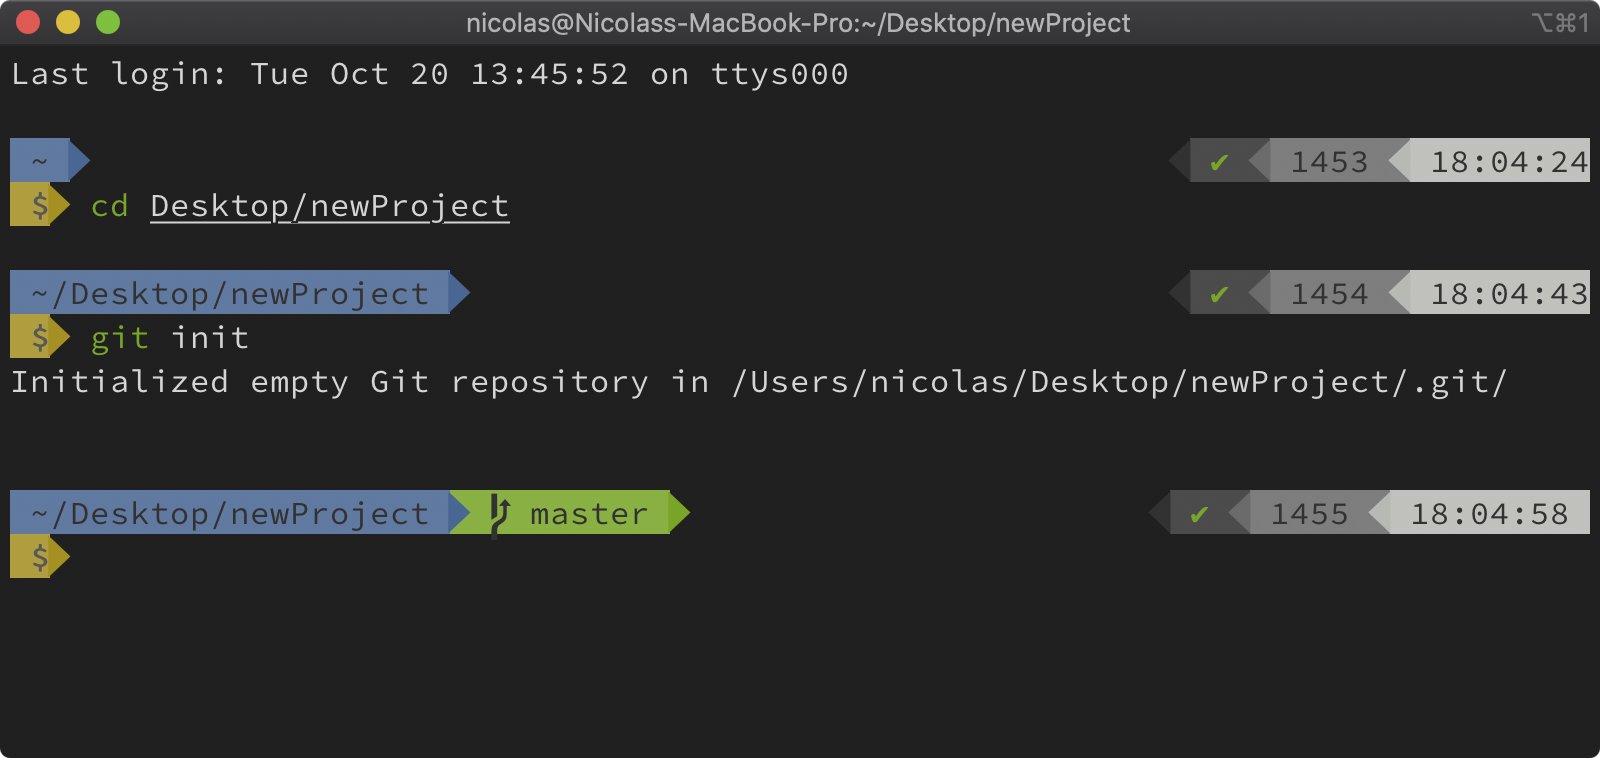
\includegraphics[width=0.9\textwidth]{src/images/gitInit.png}
	\end{exampleblock}
\end{frame}

\begin{frame}[<+->]{Ejemplo A}  
	Una vez que tenemos cambios que queramos comprometer, los podemos organizar en el \emph{staging area} \textcolor{UBCgrey}{(separar cambios en distintos \emph{commits}, por ejemplo)}
	\begin{exampleblock}{Staging}
			\centering
			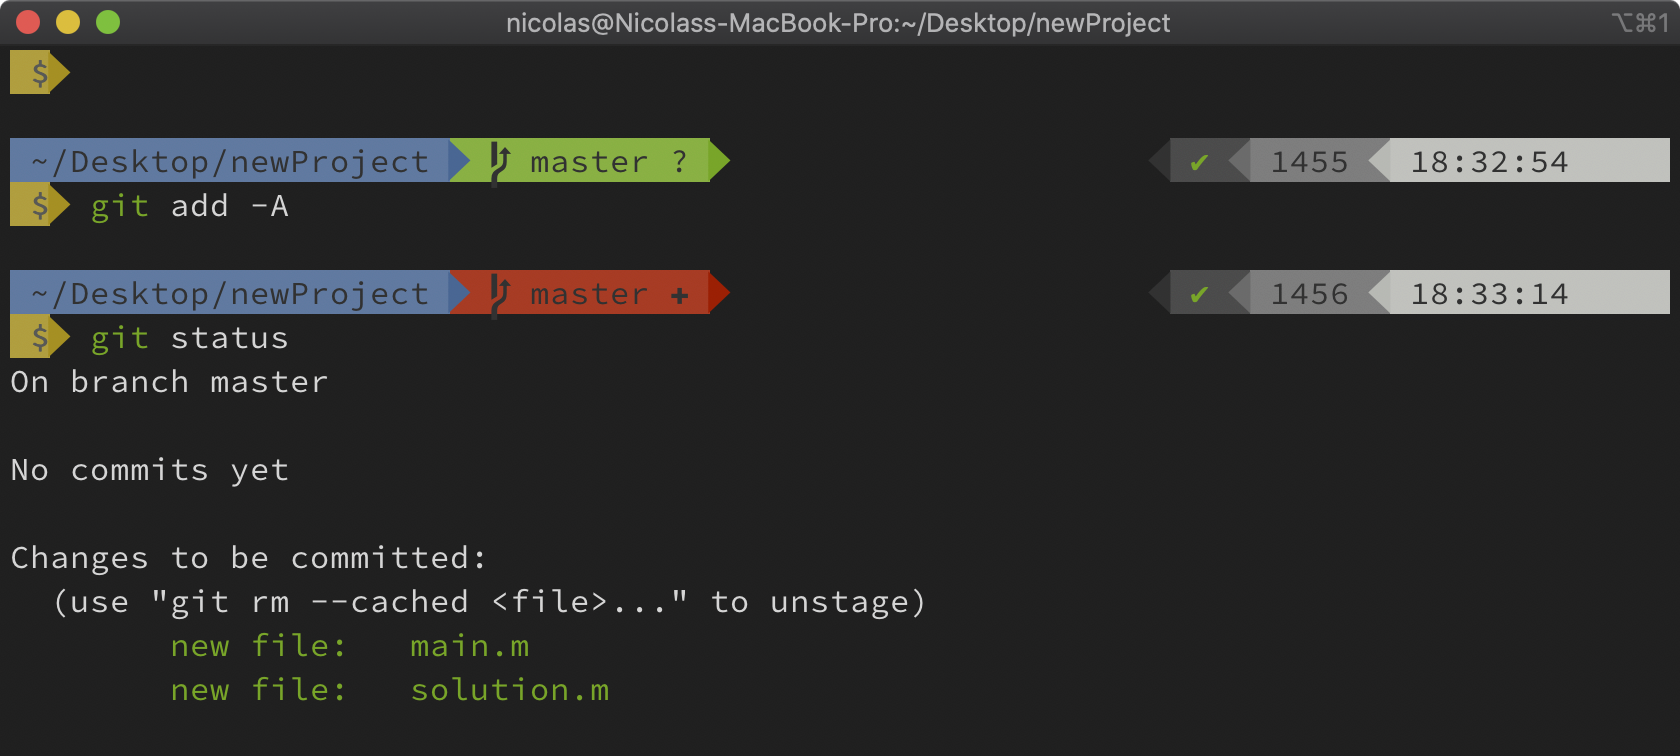
\includegraphics[width=0.9\textwidth]{src/images/gitAddStatus.png}
	\end{exampleblock}
\end{frame}

\begin{frame}[<+->]{Ejemplo A}  
	Una vez que ejecutamos el \emph{commit}, solos los cambios en el \emph{staging area} quedarán registrados.
	\begin{exampleblock}{Commit}
			\centering
			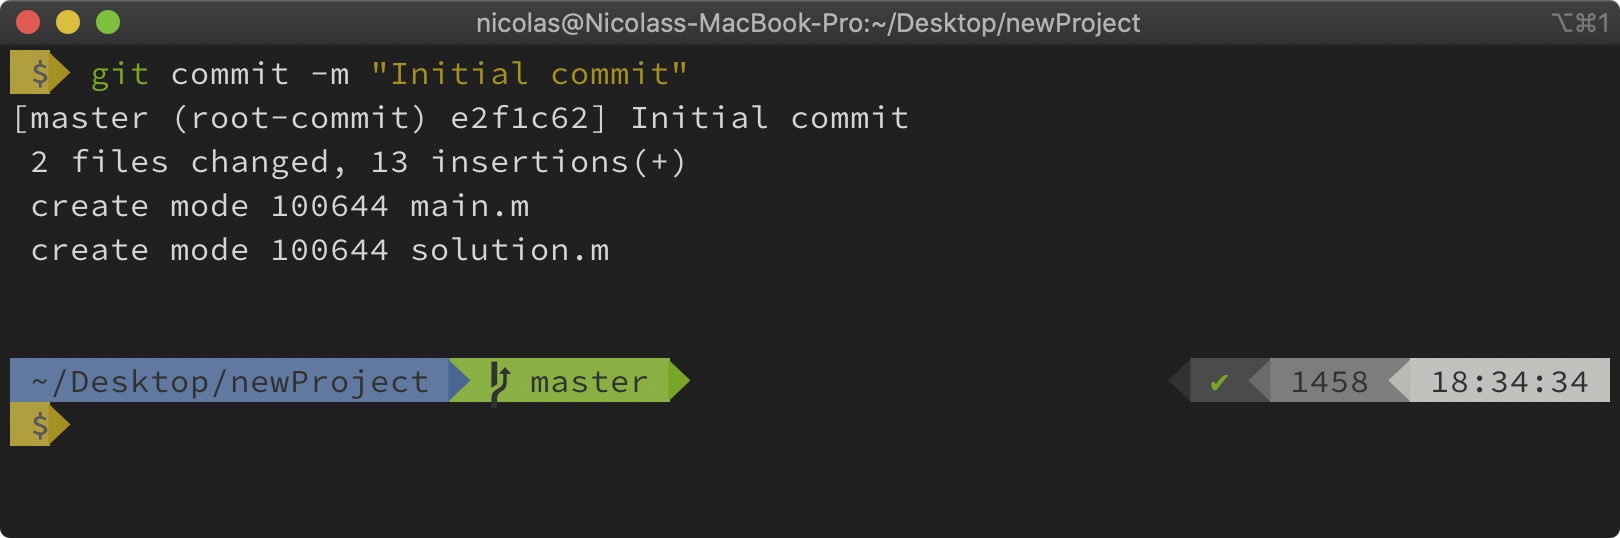
\includegraphics[width=0.9\textwidth]{src/images/gitCommit.png}
	\end{exampleblock}
\end{frame}

\begin{frame}[<+->]{Ejemplo A}
	\begin{exampleblock}{Segundo commit y git log}
			\centering
			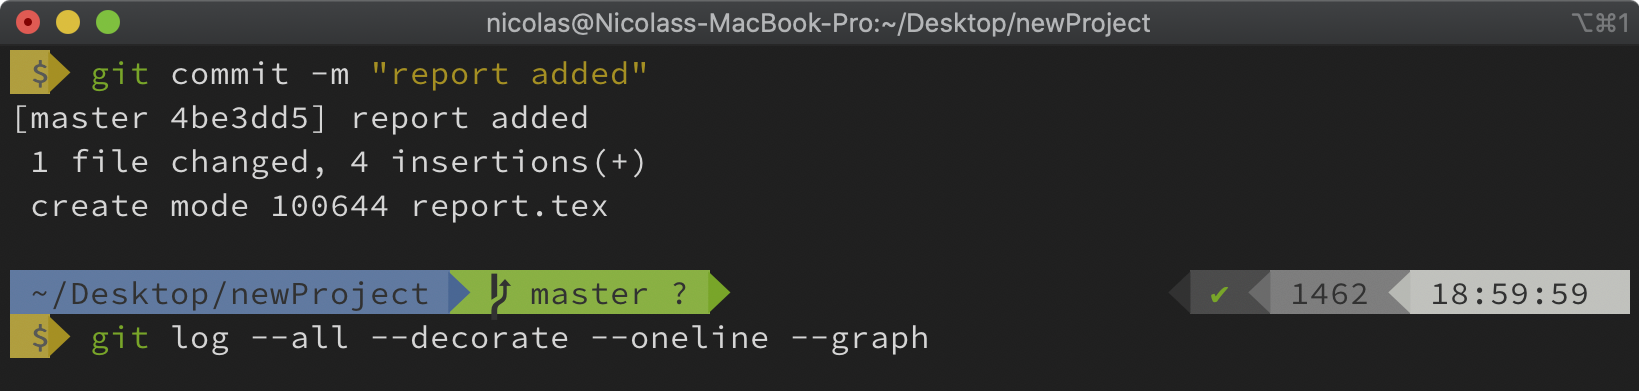
\includegraphics[width=0.9\textwidth]{src/images/gitCommit2.png}
			\vspace{0.5cm}
			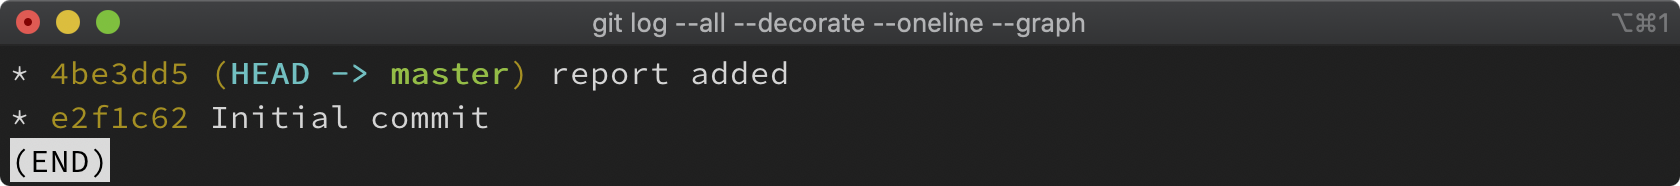
\includegraphics[width=0.9\textwidth]{src/images/gitLog.png}
	\end{exampleblock}
\end{frame}

\begin{frame}[<+->]{Ejemplo A}
	\begin{exampleblock}{Nueva rama: git branch + git checkout}
		Ahora creamos la rama ``Opcionales'' en donde cambiaremos los parametros

			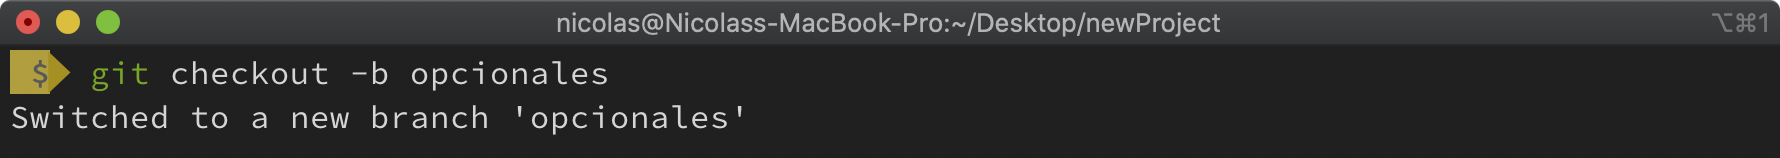
\includegraphics[width=0.9\textwidth]{src/images/gitCheckoutB.png}\\

		Una vez que hacemos los cambio en el archivo ``main.m'' hacemos el \emph{staging} y \emph{commit}

			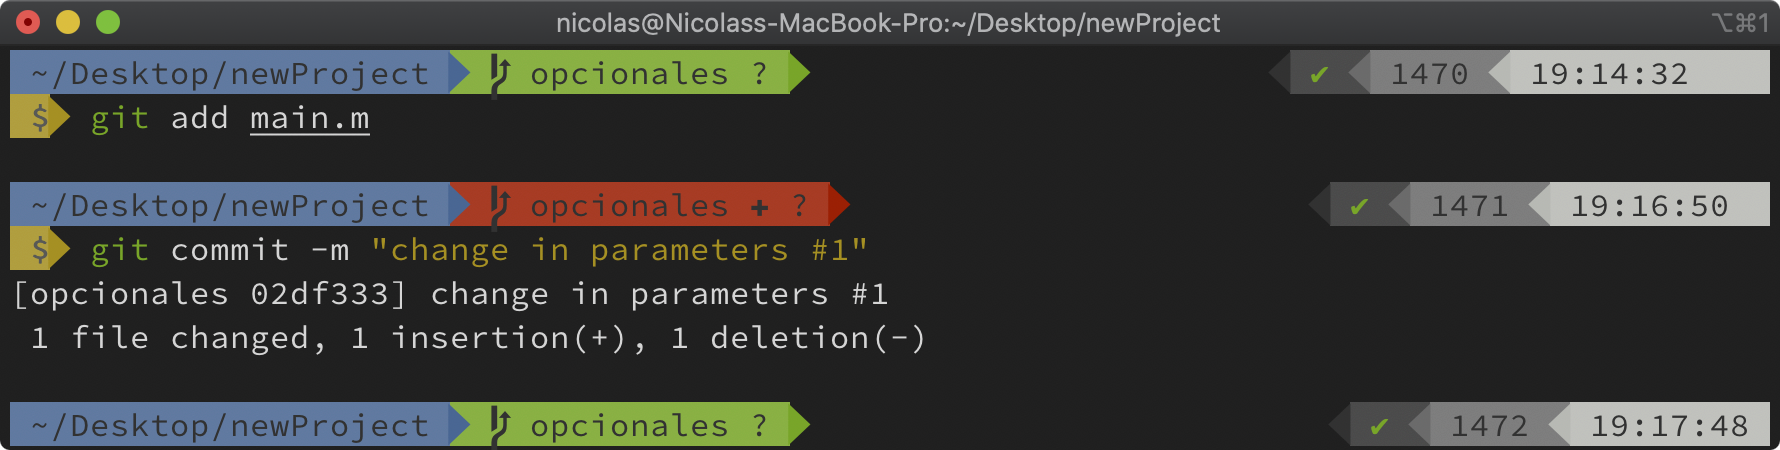
\includegraphics[width=0.9\textwidth]{src/images/gitCommitInBranch.png}
	\end{exampleblock}
\end{frame}

\begin{frame}[<+->]{Ejemplo A}
	\begin{exampleblock}{Git diff}
		Para visualizar los cambios que hicimos existe el comando \emph{git diff}, seguido por identificadores de los \emph{commits} a comparar y opciones del comando 

		\centering{
			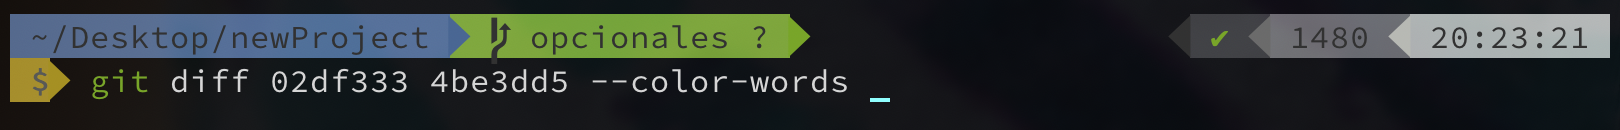
\includegraphics[width=0.9\textwidth]{src/images/gitDiffTerminal.png}

			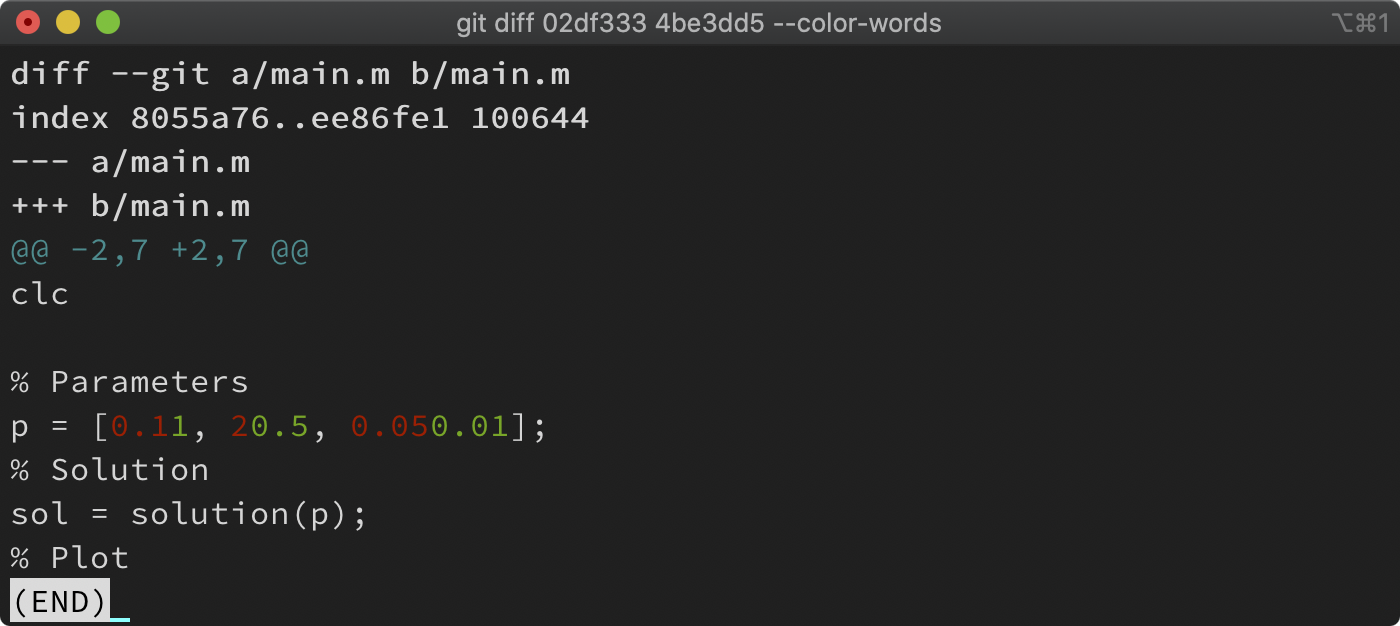
\includegraphics[width=0.7\textwidth]{src/images/gitDiff.png}}
	\end{exampleblock}
\end{frame}

\begin{frame}[<+->]{Ejemplo A}
	\begin{exampleblock}{Git checkout}
		Ahora nos acabamos de dar cuenta de un error en \emph{solucion.m}. Dado que el error involucra a todo el repositorio, es mejor resolver el problema en ``master''. Para ello tenemos que saltar de rama 
		
		{\centering
			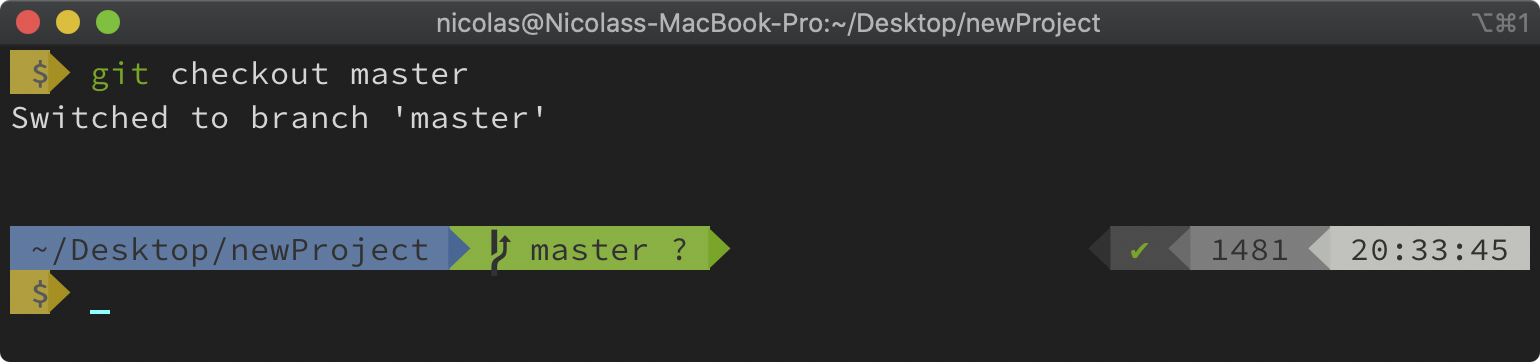
\includegraphics[width=0.9\textwidth]{src/images/gitCheckoutMaster.png}
			}\\
		
			\onslide<+->{Una vez resuelto el problema, y comprometidos los cambios, podemos seguir trabajando en nuestra rama opcionales} \onslide<+->{\alert{... excepto por...}}
	\end{exampleblock}
\end{frame}

\begin{frame}[<+->]{Ejemplo A}
	\begin{exampleblock}{git merge}
		El arreglo en ``master'' no esta disponible en ''opcionales''. Para llevar la linea de ``master'' a ``opcionales'' nos cambiamos a la segunda y hacemos un \emph{merge} con la primera.\\

		\centering{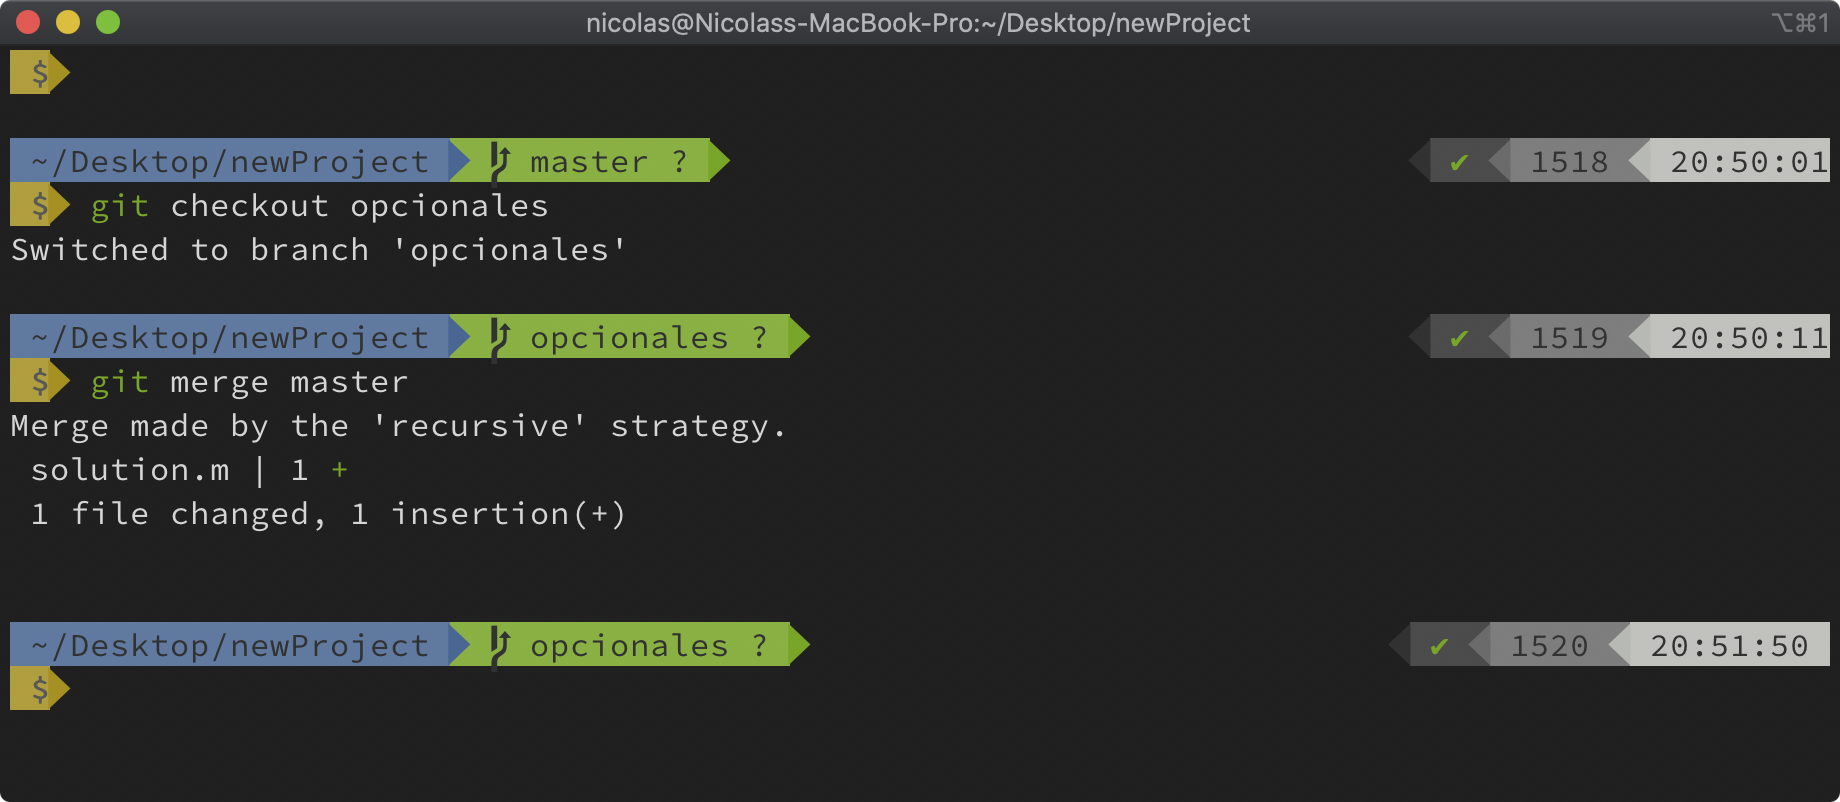
\includegraphics[width=0.8\textwidth]{src/images/gitMerge.png}}
	\end{exampleblock}
\end{frame}

\begin{frame}[<+->]{Ejemplo A}
	\begin{exampleblock}{Visualización del arbol git}
		\medskip
			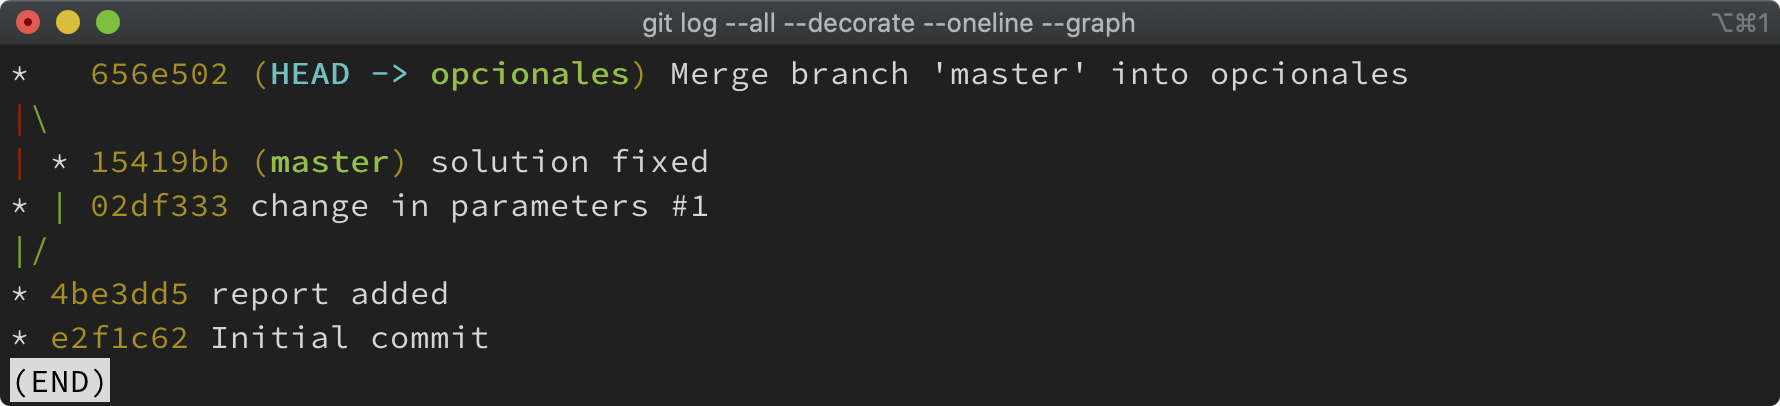
\includegraphics[width=0.8\textwidth]{src/images/gitLog2.png}

		\medskip
		Ahora podemos evaluar nuestras pruebas en ``opcionales''. Si los cambios nos gustan, los podemos incluir en nuestra rama ``master'' haciendo un \emph{merge}, esta vez de ``opcionales'' a ``master''.
	\end{exampleblock}
\end{frame}

\begin{frame}[<+->]{Ejemplo A}
	\begin{exampleblock}{Merge y branch -d}
		
		Una vez que ejecutamos el \emph{merge}, eliminar la rama ``opcionales'' (\$ \emph{git branch -d opcionales}) no elimina la información de los commits hechos en ella
		\medskip

			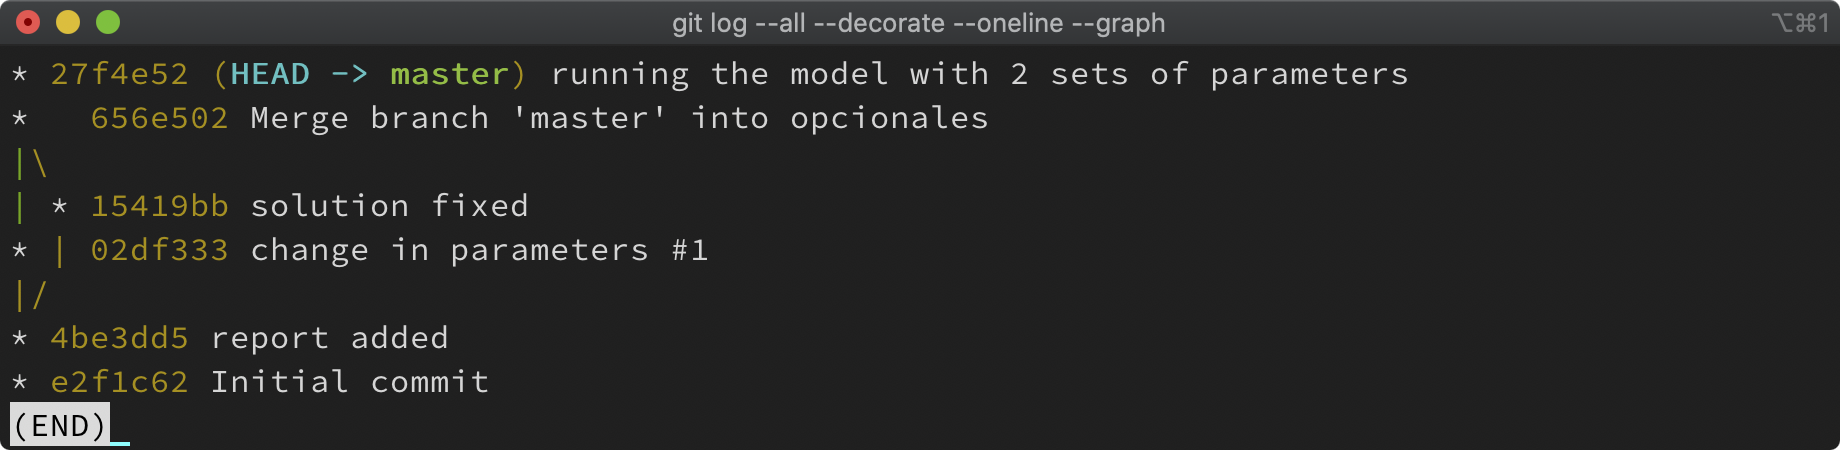
\includegraphics[width=0.8\textwidth]{src/images/gitLogNobranch.png}

		\medskip

		\onslide<+->{Ahora nuestro árbol está limpio y tenemos una visualización de cómo los cambios sucedieron}
	\end{exampleblock}
\end{frame}

\begin{frame}{Comandos git y algunos comentarios}
	\begin{columns}[T, onlytextwidth]
		\column{0.5\textwidth}
		\begin{itemize}[<+->]
			\item Los comandos que utilizamos tienen opciones que los hacen muy versátiles
			\vfill \item Git es más inteligente de lo que usualmente pensamos
			\vfill \item Cuando hay conflictos git no nos dejará hacer los cambios sin resolverlos
			\vfill \item Cuando hay información no guardada en una rama, git no nos permitirá saltar a otra \textcolor{UBCgrey}{(para esto existe el comando stash)}
			\vfill \item La mayoría de los comandos Git agregan información \textcolor{UBCgrey}{(muy rara vez la eliminan)}
		\end{itemize}
		\column{0.5\textwidth}
		\begin{itemize}[<+->]
			\item \textbf{git init}: inicializar un repositorio
			\vfill \item \textbf{git add}: presentar cambios en el escenario
			\vfill \item \textbf{git commit}: registrar los cambios
			\vfill \item \textbf{git status}: estado del repositorio
			\vfill \item \textbf{git log}: listado de \emph{commits}
			\vfill \item \textbf{git diff}: diferencias entre un \emph{commit} y otro.
			\vfill \item \textbf{git branch}: crear una nueva rama.
			\vfill \item \textbf{git checkout}: saltar de una rama a otra.
			\vfill \item \textbf{git merge}: mezclar ramas.
		\end{itemize}
	\end{columns}
\end{frame}

\begin{frame}[standout]{Ejemplo A}
	Preguntas?
\end{frame}

%--------------------------------------------------------------------------------------
%										SECCION: UI
%--------------------------------------------------------------------------------------
\section{Interfaces de usuario, ``la nube'' y redes sociales}

\begin{frame}[<+->]{\secname}
	\begin{itemize}
		\item Usar git en la línea de comando puede tomar algún tiempo.
		\vfill \item Las interfaces de usuario facilitan el proceso, pero involucran preferencias personales.
		\vfill \item Una de las UI populares es VS Code de Microsoft
		\begin{itemize}
			\item Integración Git desde su instalación 
			\item Variados lenguages de programación y herramientas que facilitan la escritura de código.
			\item Marketplace con extensiones gratuitas 
		\end{itemize}
		\begin{exampleblock}{VS code}
			Desde VS code se puede utilizar y compilar \LaTeX ~ y markdown. Se puede utilizar Matlab, python y R. Se puede tener un sistema de punteros \emph{TODO} y \emph{FIXME}. Sistemas de corrección ortográfico (tanto para texto como código), sistema de brackets colorizados, etc
		\end{exampleblock}
	\end{itemize}
\end{frame}

\begin{frame}[<+->]{GUI's}
	\begin{figure}[H]
		\centering
		\caption{VScode, git diff}
		\vspace{-0.5cm}
		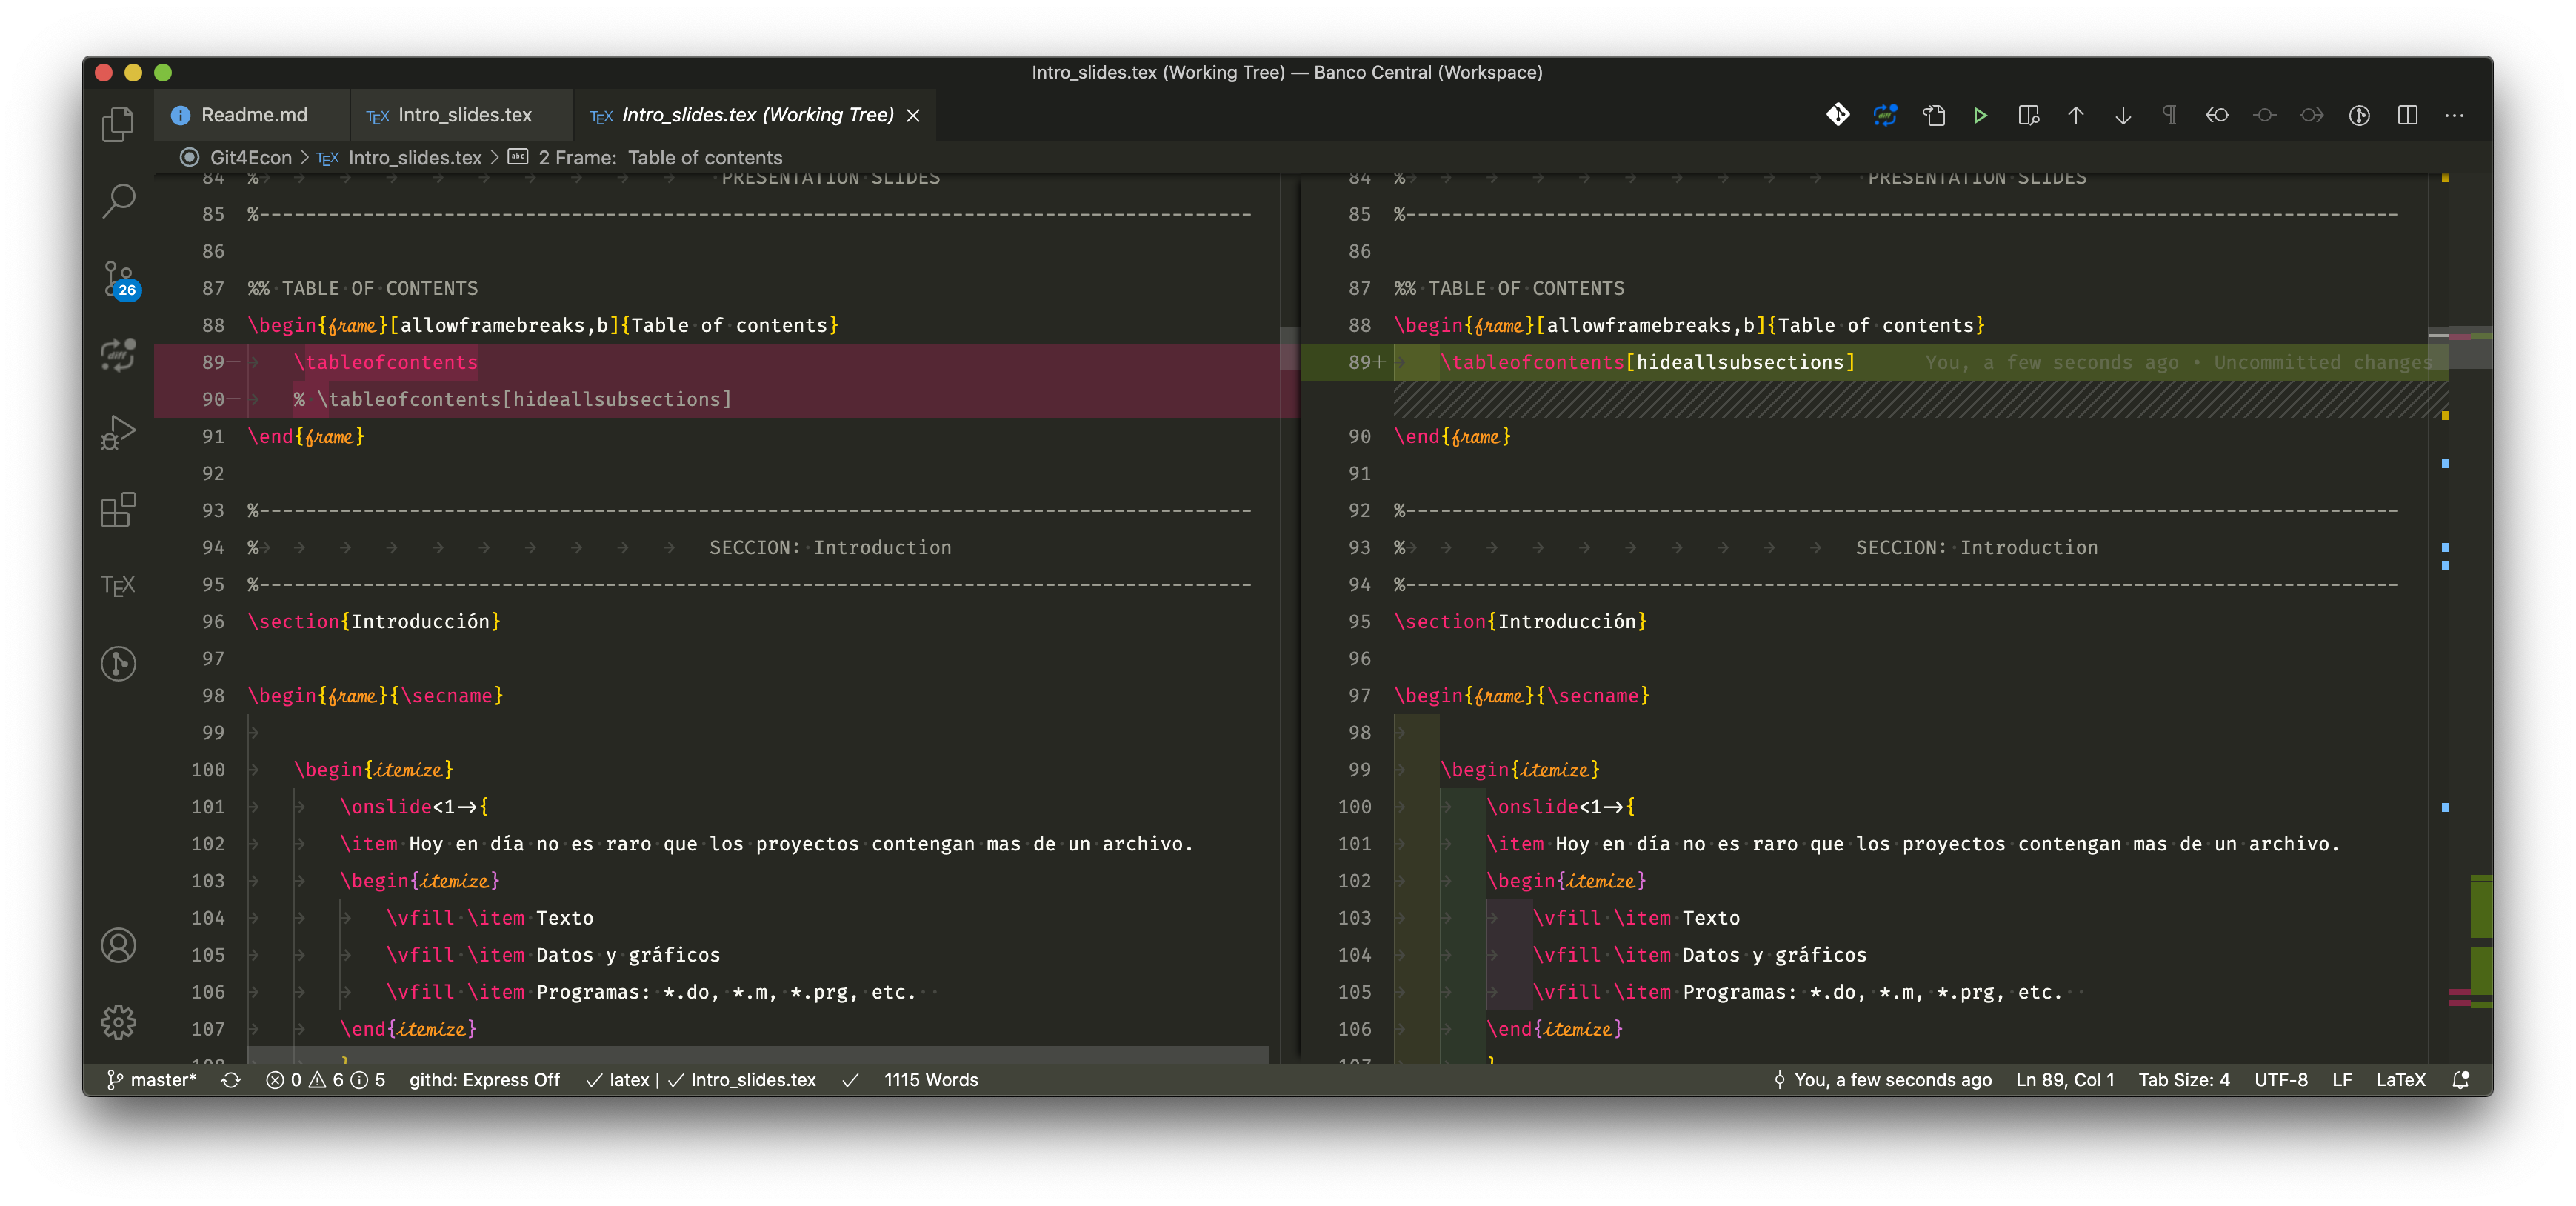
\includegraphics[width=\textwidth]{src/images/VScodeDiff.png}
	\end{figure}
\end{frame}

\begin{frame}[<+->]{GUI's}
	\begin{figure}[H]
		\centering
		\caption{VScode, file history}
		\vspace{-0.5cm}
		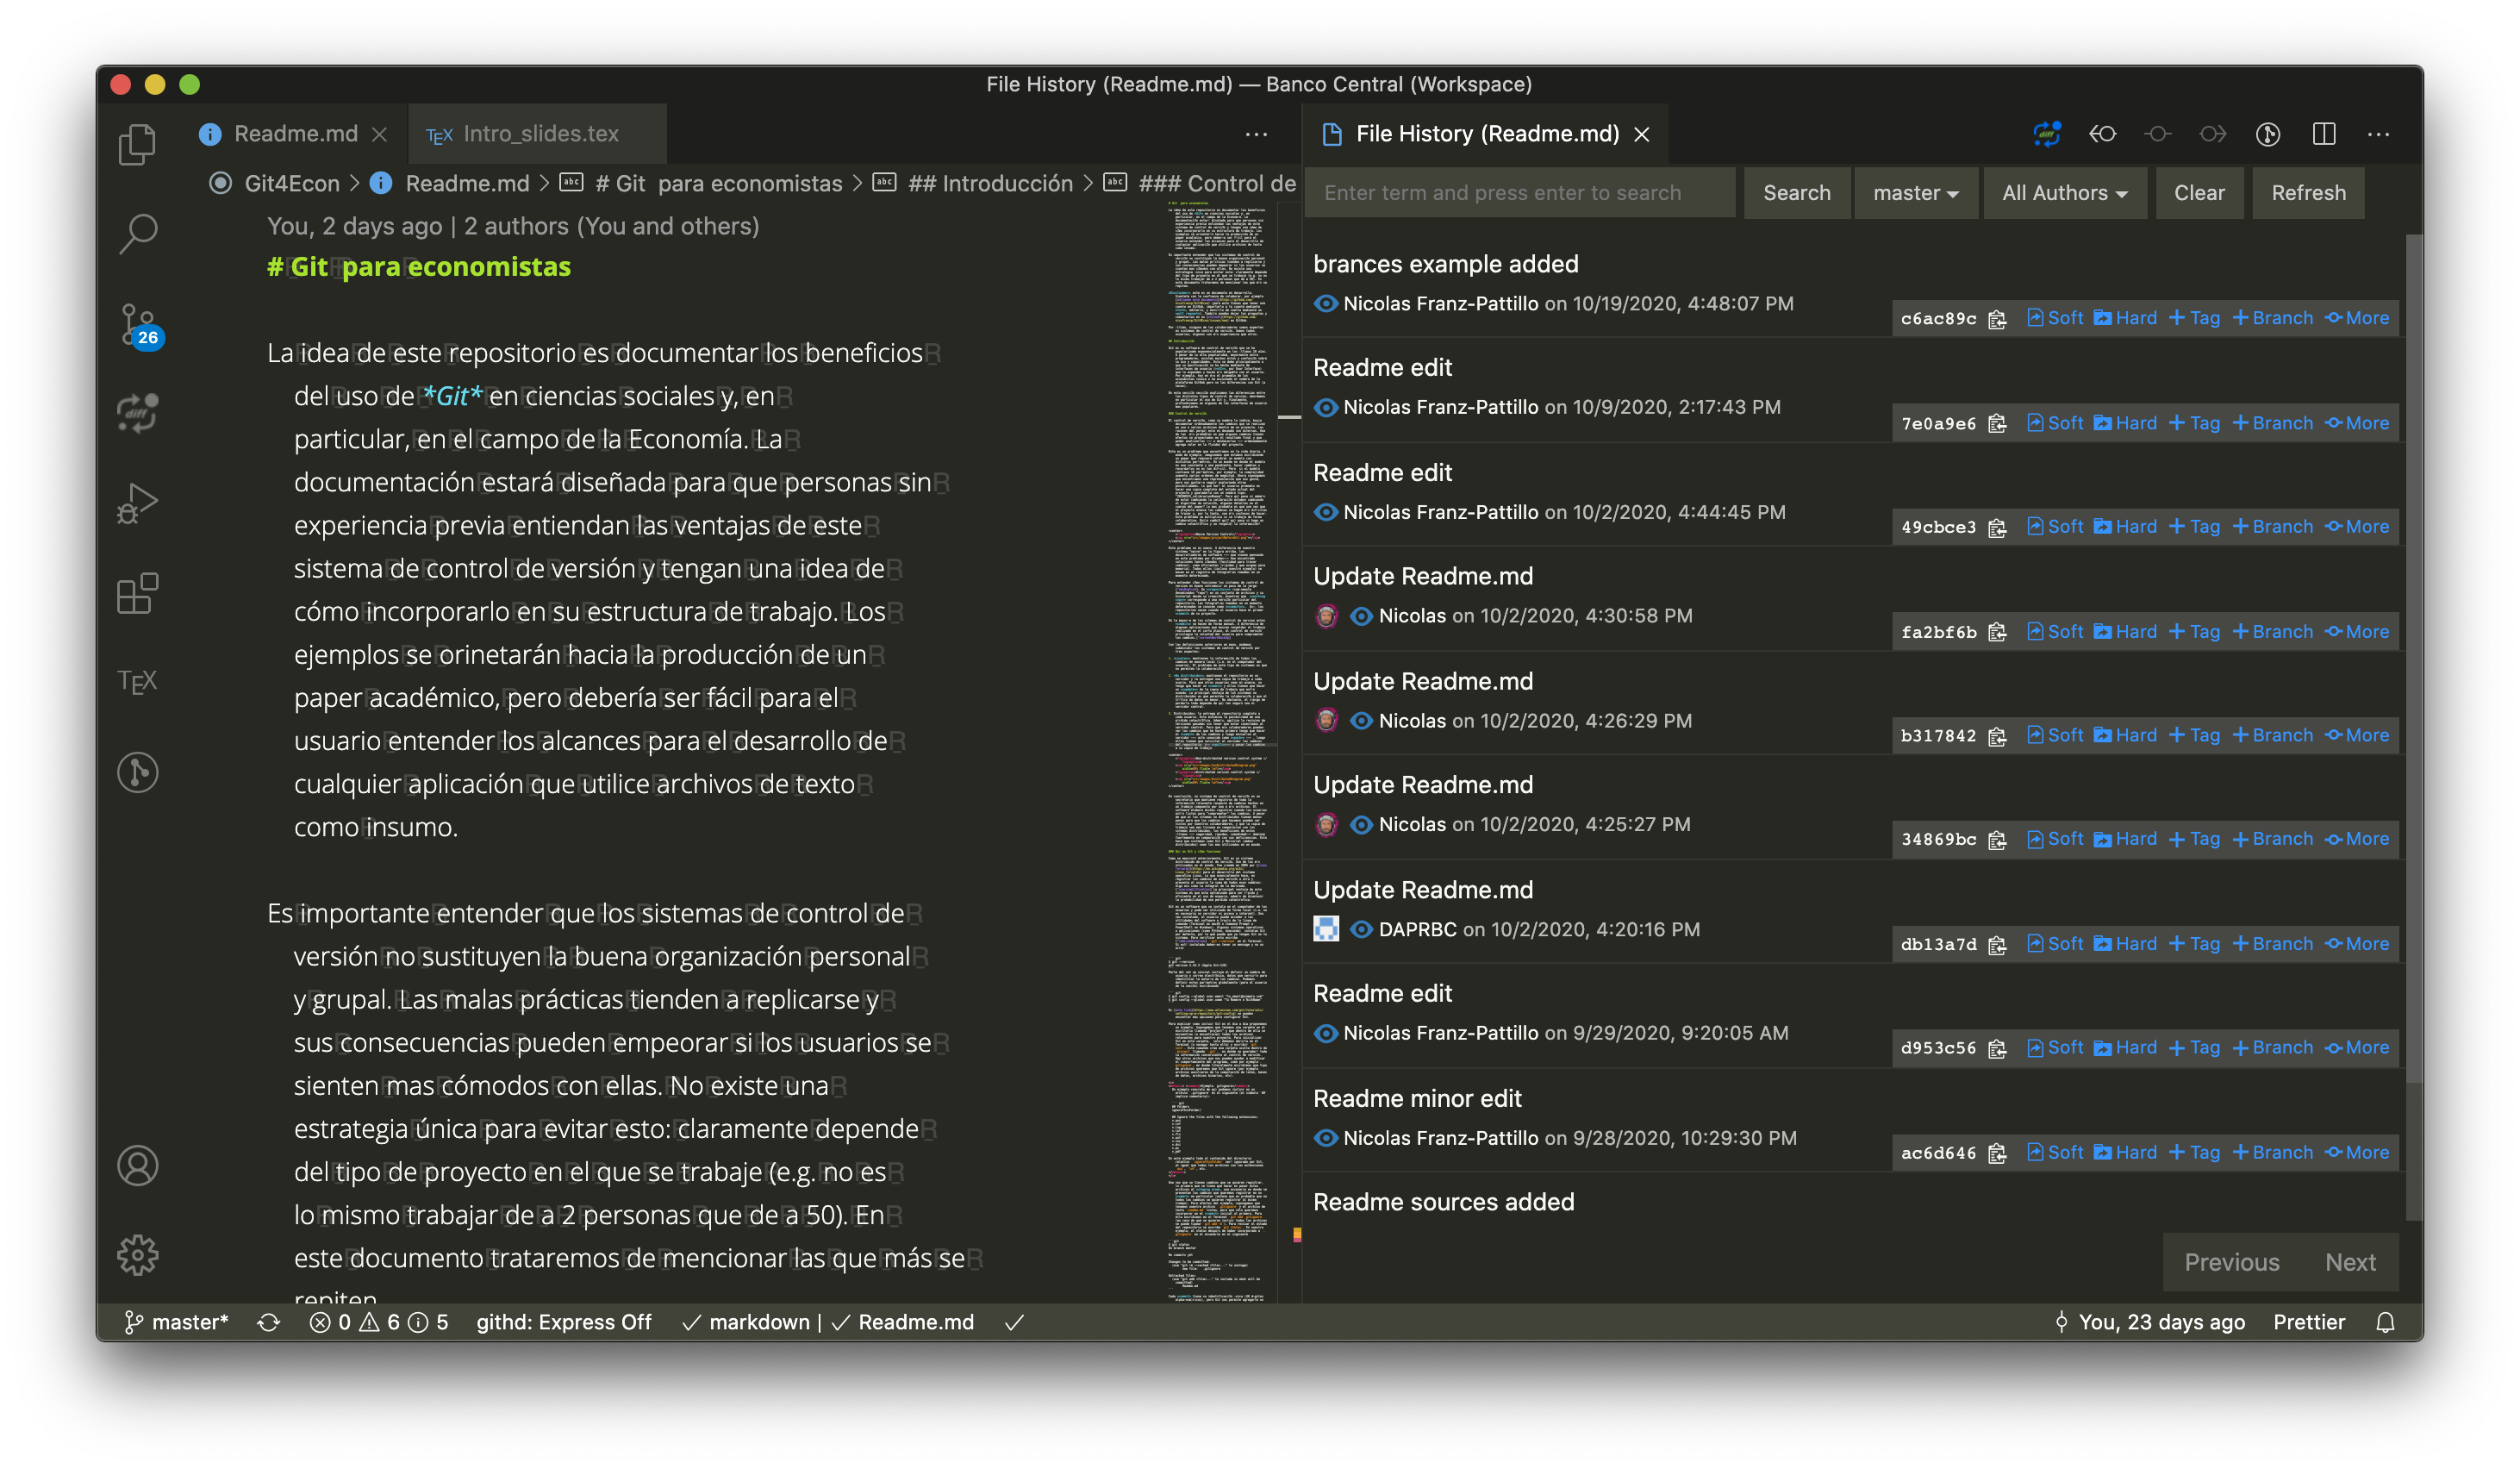
\includegraphics[width=0.9\textwidth]{src/images/VScodeFileHistory.png}
	\end{figure}
\end{frame}

\begin{frame}[<+->]{GUI's}
	\begin{figure}[H]
		\centering
		\caption{VScode, git diff (seleccionando commits)}
		\vspace{-0.5cm}
		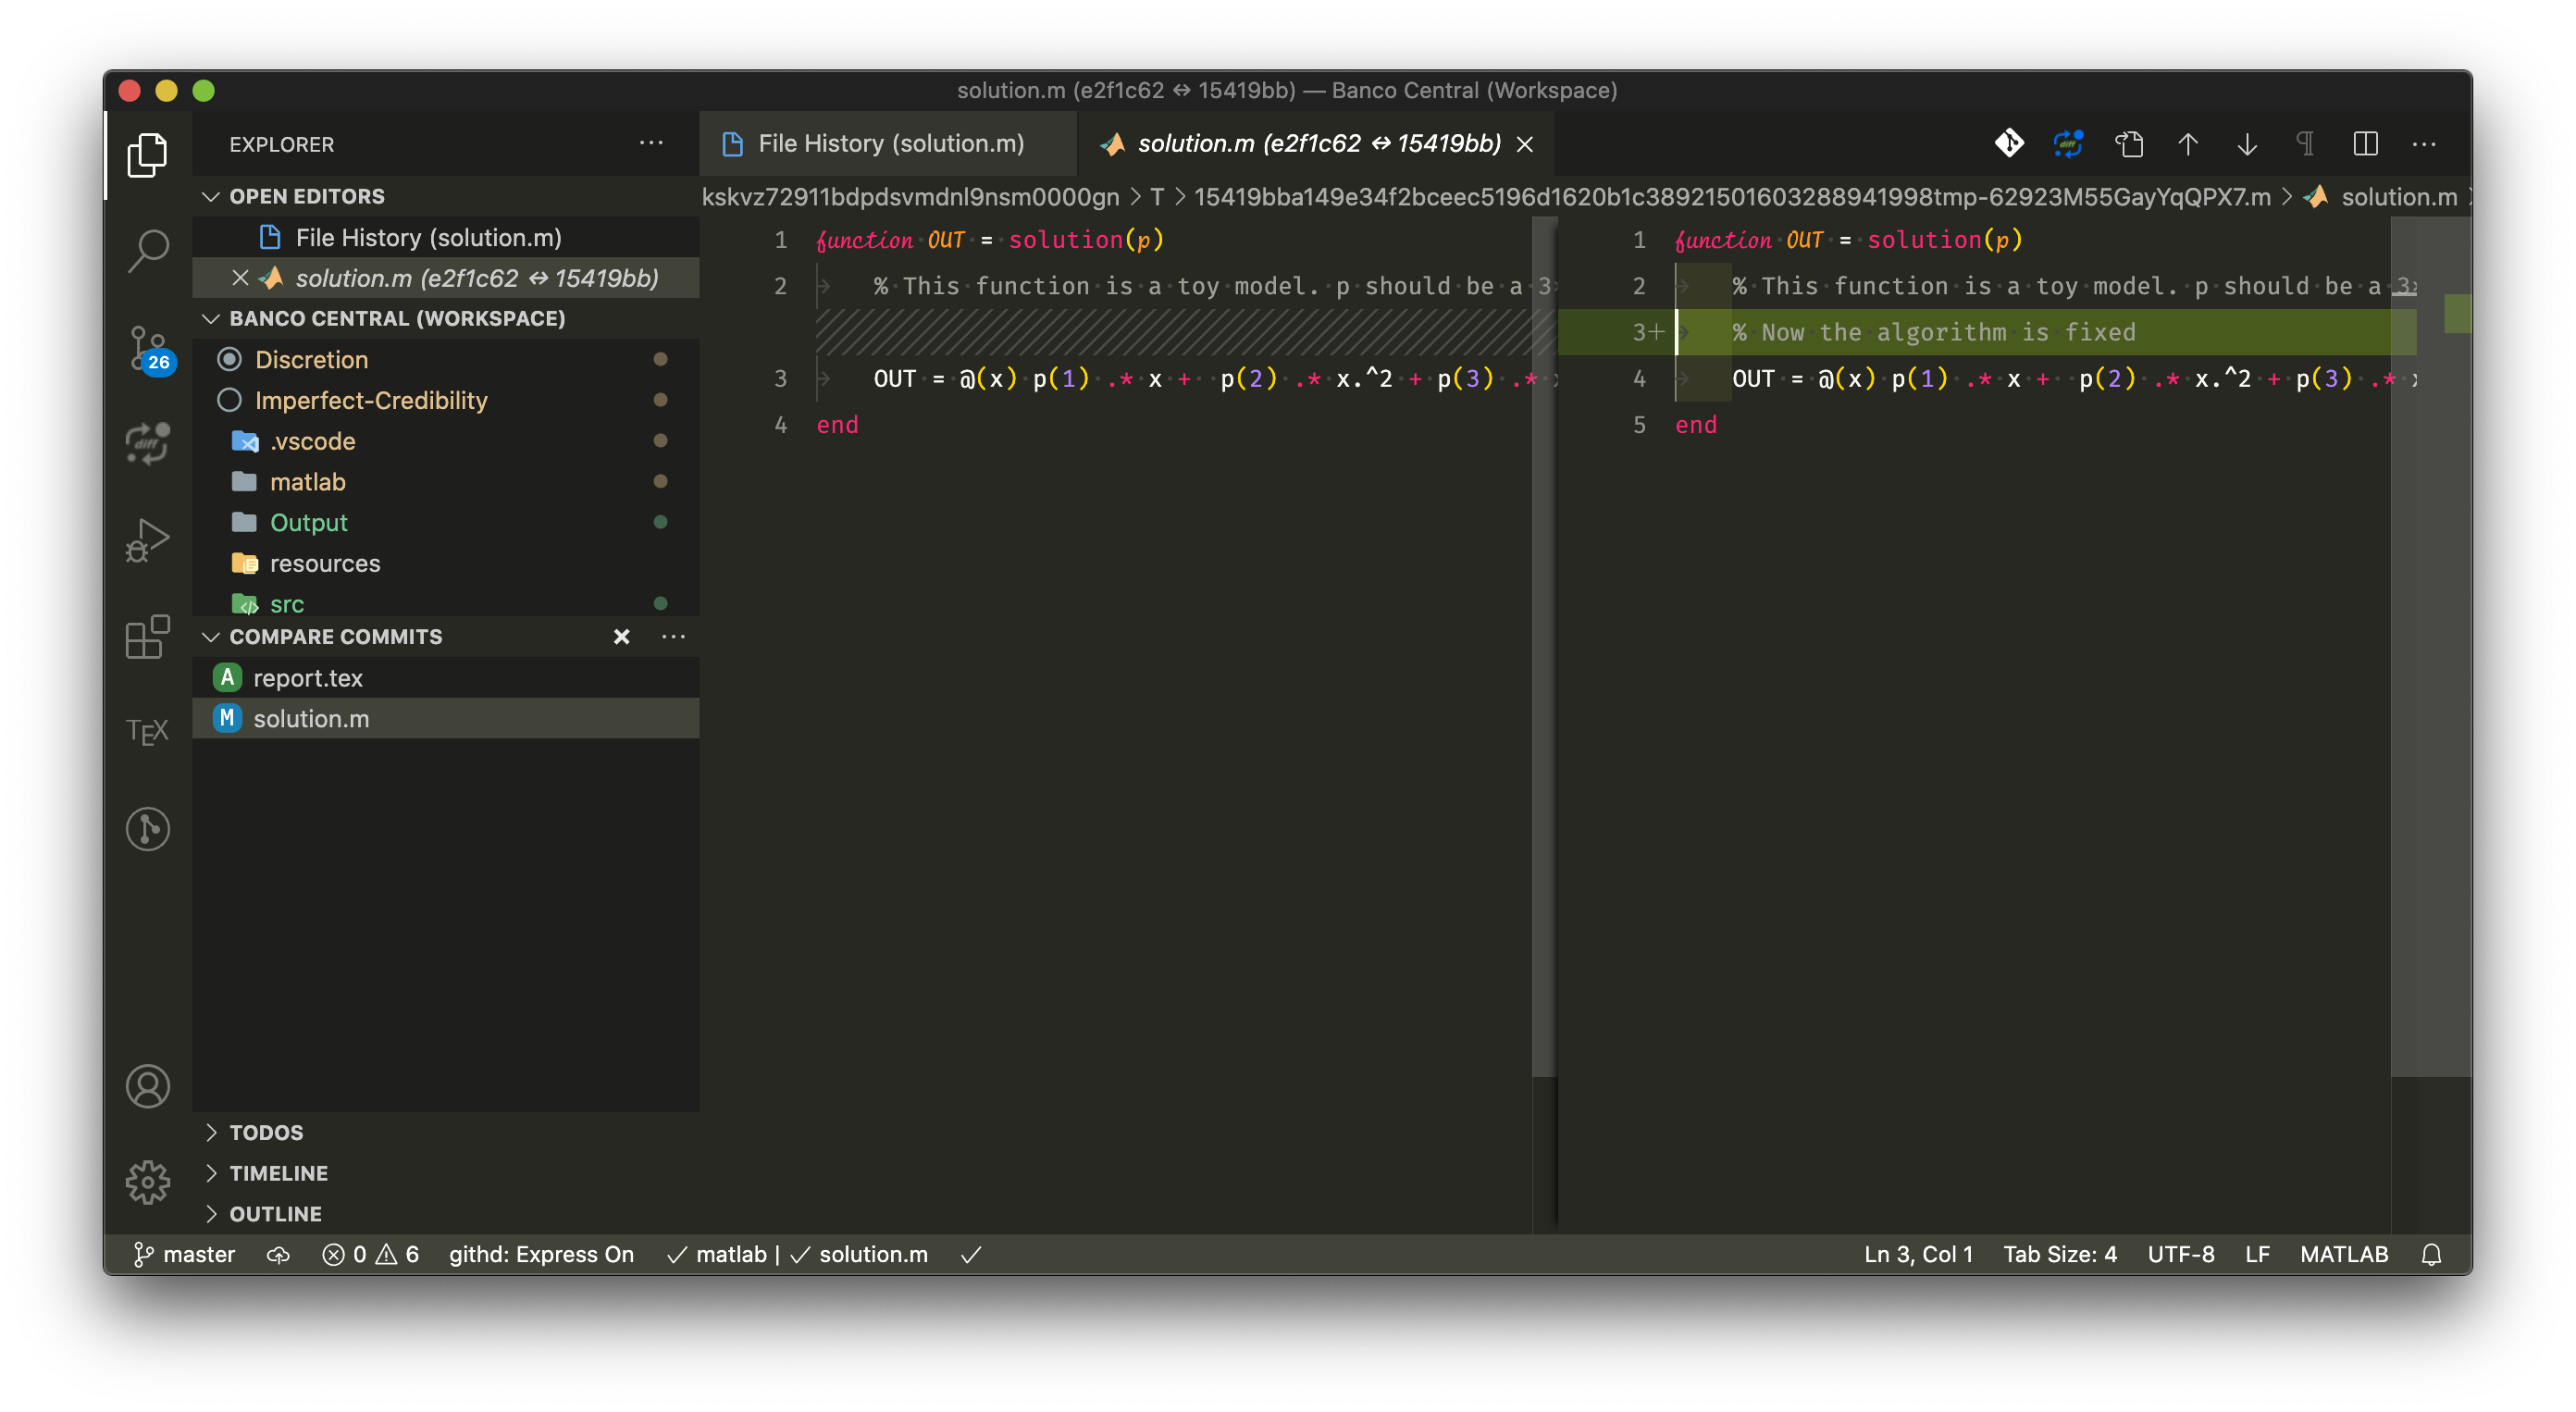
\includegraphics[width=0.9\textwidth]{src/images/VScodeCompareCommits.png}
	\end{figure}
\end{frame}

\begin{frame}[<+->]{GUI's}
	\begin{figure}[H]
		\centering
		\caption{VScode, git diff (seleccionando commits)}
		\vspace{-0.5cm}
		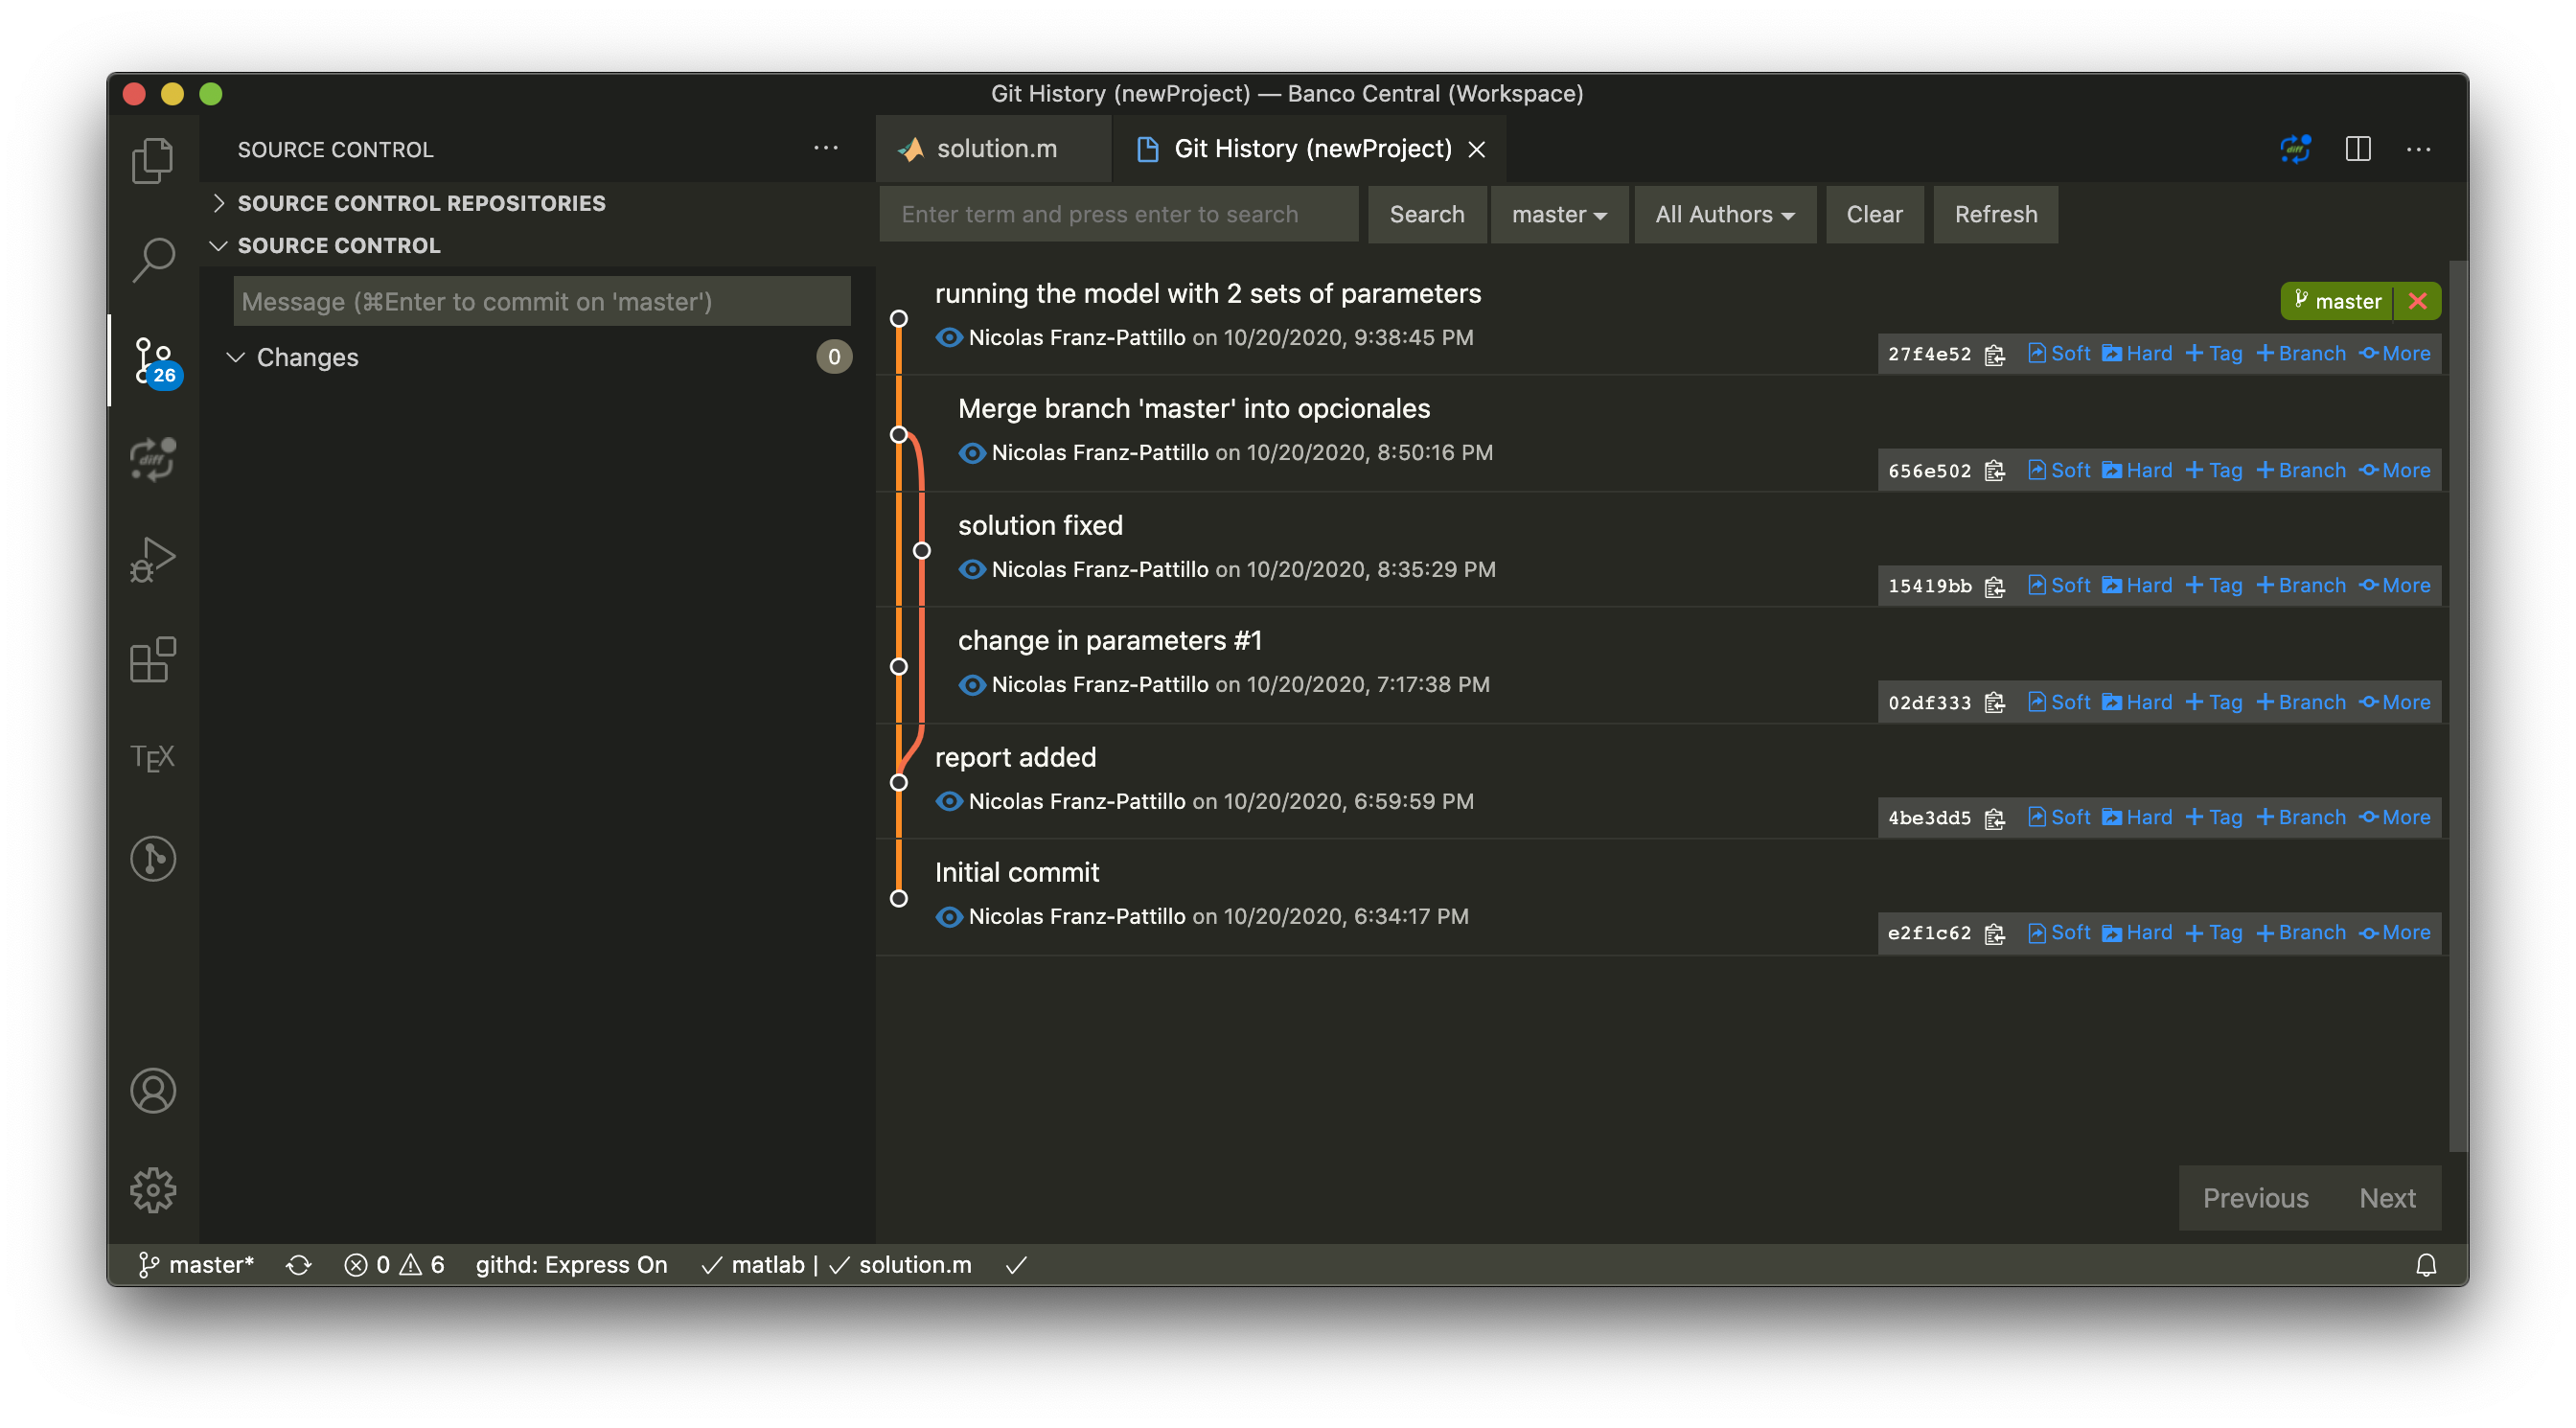
\includegraphics[width=0.9\textwidth]{src/images/VScodeLogGraph.png}
	\end{figure}
\end{frame}

\begin{frame}[<+->]{Colaboración con Git}
	\begin{itemize}
		\item Anteriormente mencionamos que git no requiere servidores.
		\vfill\item En teoría, podríamos compartir un repositorio utilizando un disco duro en común
		\vfill\item También se pueden crear permisos de lectura y escritura (ver documentación de \href{https://git-scm.com/docs/git-init}{git init})
		\vfill\item No obstante, un servidor git permite crear un espacio común y seguro!
		\vfill\item Git ocupa los siguientes protocolos de comunicación:
		\begin{enumerate}
			\item Local
			\item HTTP y HTTPS
			\item SSH
			\item GIT 
		\end{enumerate}
	\end{itemize}
\end{frame}

\begin{frame}[<+->]{``La nube'' y redes sociales}
	\begin{itemize}
		\item ``La nube'' no es mas que un grupo de servidores
		\vfill\item Para colaborar con git sólo nos hace falta aprender los siguentes comandos
		\begin{enumerate}
			\vfill\item git remote
			\vfill\item git clone
			\vfill\item git pull (git fetch + git commit)
			\vfill\item git push
		\end{enumerate}
	\end{itemize}
\end{frame}

\begin{frame}[<+->]{``La nube'' y redes sociales}
	\begin{itemize}
		\item Sin embargo hay un componente humano que hace falta
		\vfill\item Tener la información no es lo mismo que entender la información
		\vfill \item Este espacio lo llenan las redes sociales, que permiten dar fluidez a la comunicación
		\begin{itemize}
			\vfill \item Archivos Readme y Wiki
			\vfill \item Issues
			\vfill \item Forks 
			\vfill \item Pull requests 
		\end{itemize}
		\vfill \item Las mas famosas son GitHub, GitLab y BitBucket.
		\vfill \item Se pueden intalar en redes privadas. 
	\end{itemize}
\end{frame}

\begin{frame}[<+->]{GitHub}
	\begin{figure}[H]
		\centering
		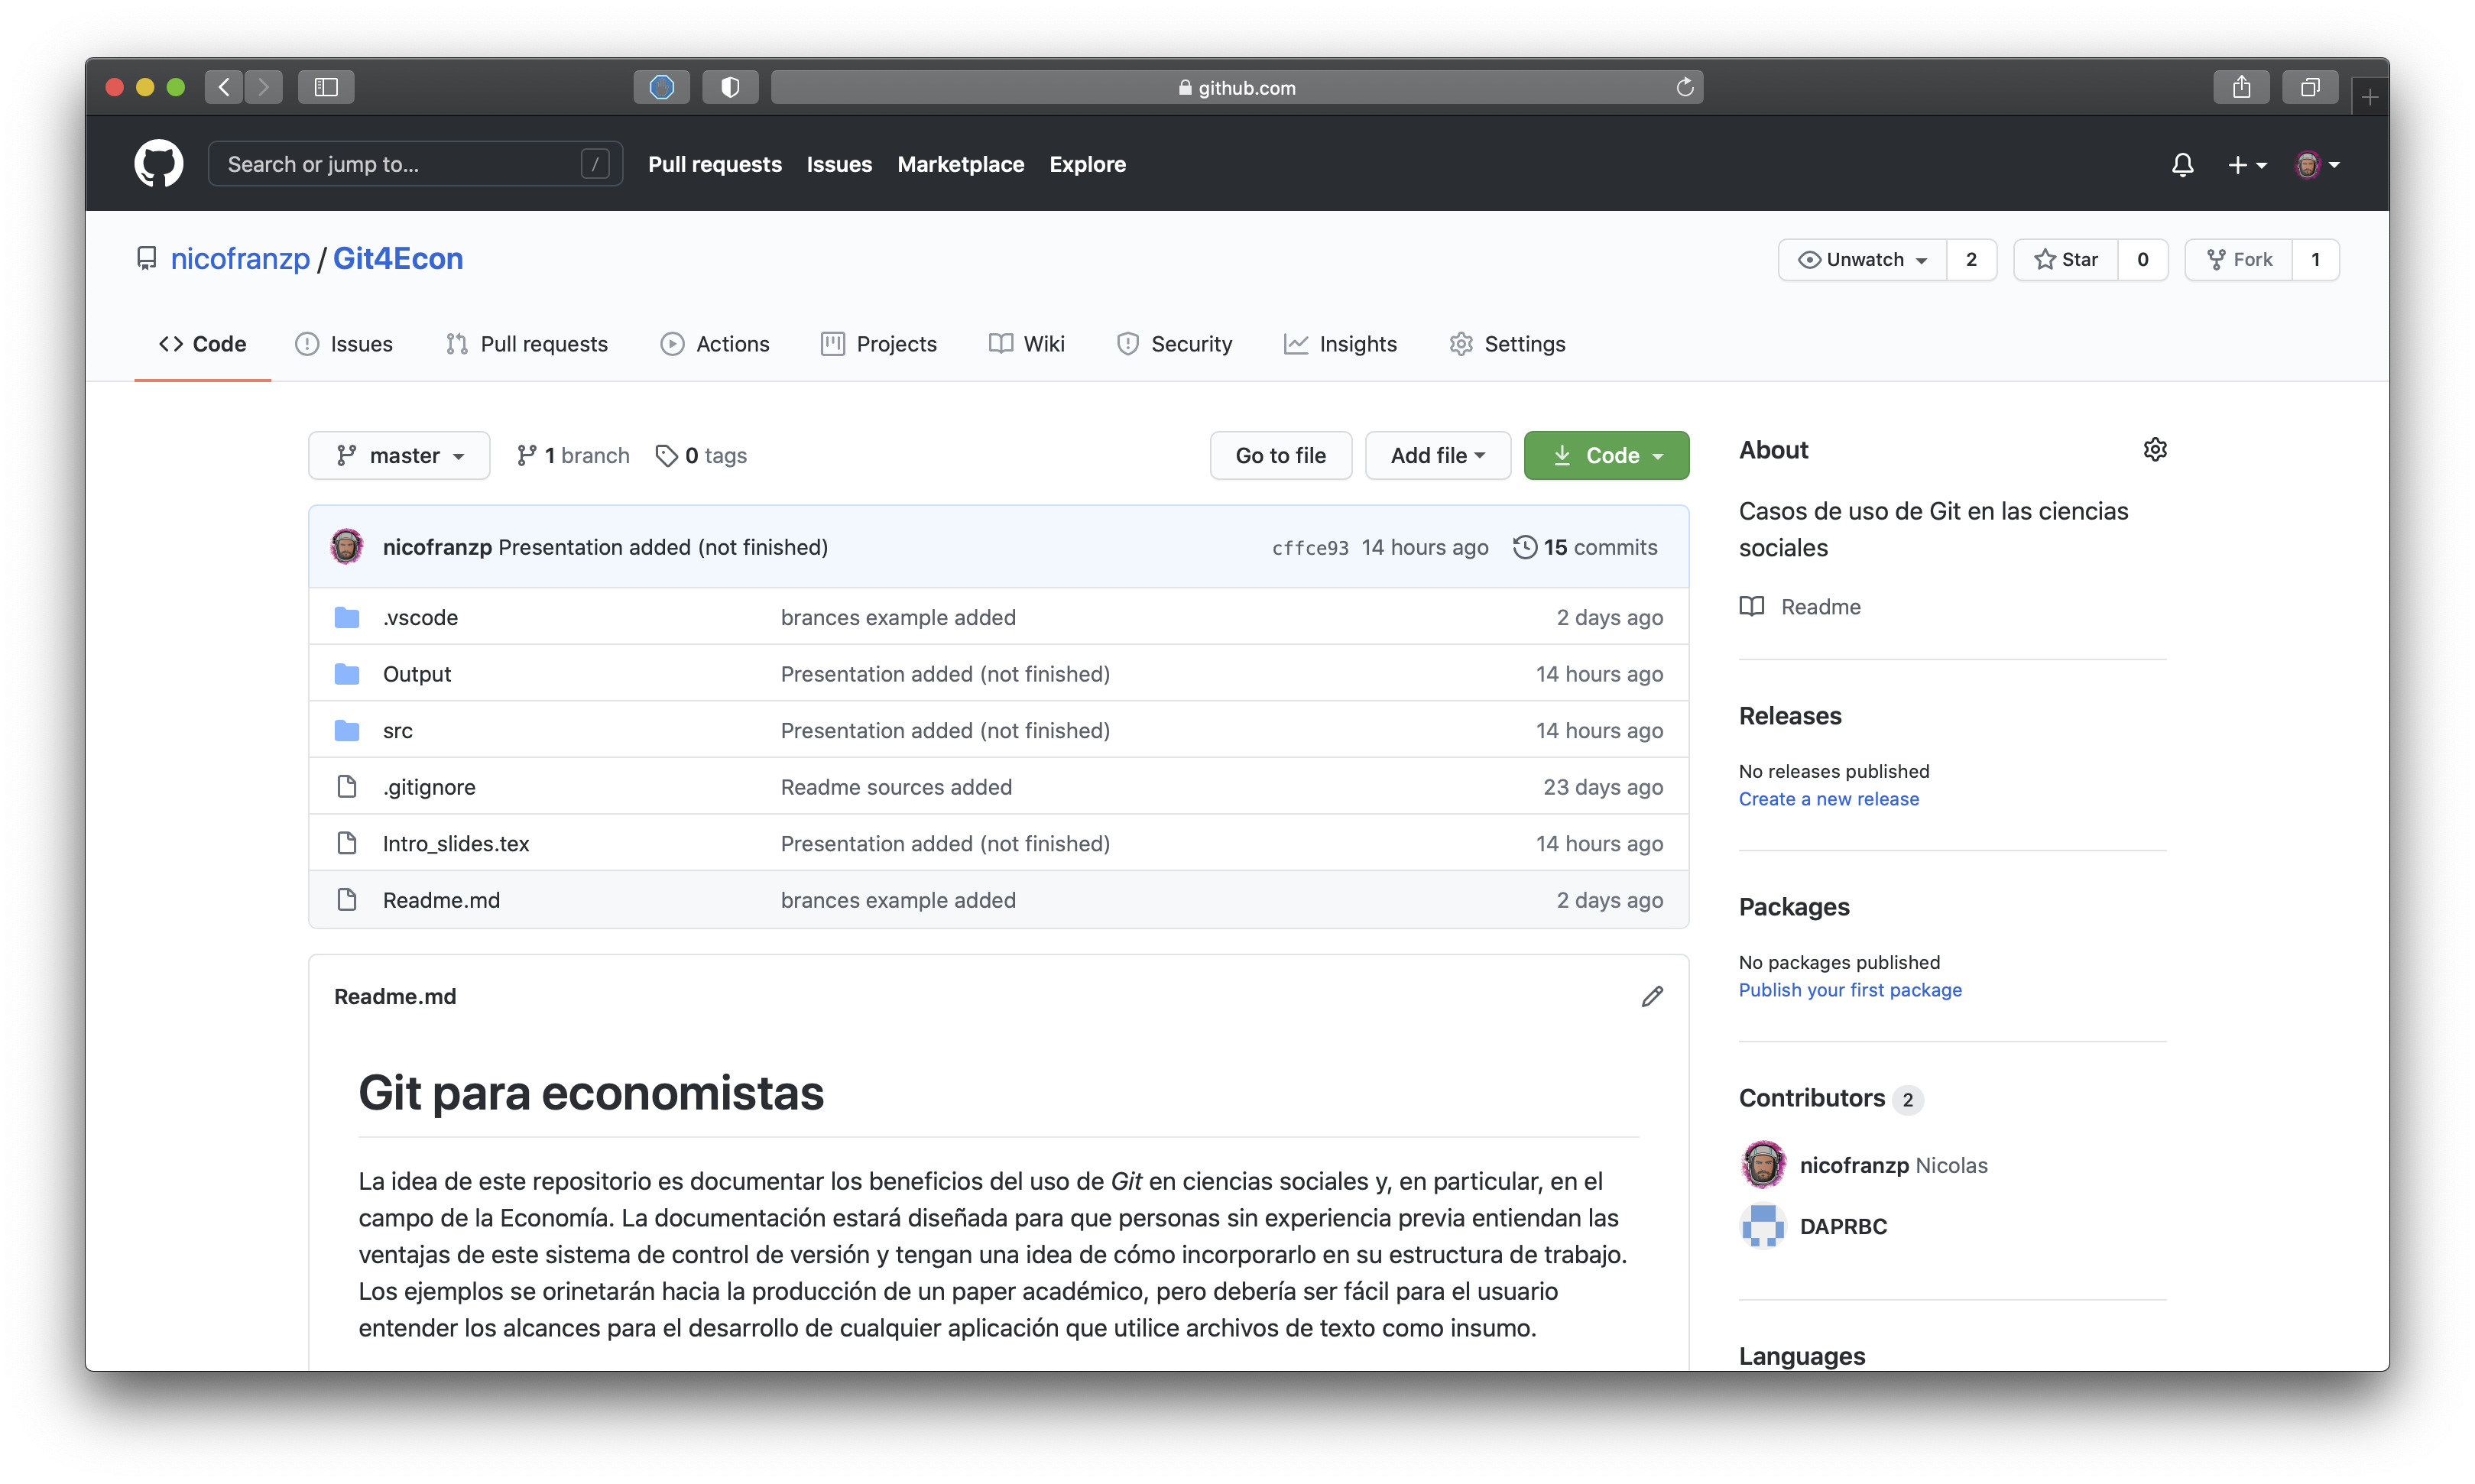
\includegraphics[width=0.9\textwidth]{src/images/gitHub.png}
	\end{figure}
\end{frame}

\begin{frame}[standout]{\secname}
	Preguntas?
\end{frame}
%--------------------------------------------------------------------------------------
%										SECCION: CONCLUSIONES
%--------------------------------------------------------------------------------------
\section{Buenas prácticas y Conclusiones}

\begin{frame}[<+->]{Comentarios finales}
	\begin{itemize}
		\item Git es un secretario que lleva registro completo del repositorio.
		\item Git no es mágico. Requiere que los equipos definan estrategias para crear ramas y resolver conflictos.
		\vfill\item Su utilidad aumenta exponencialmente cuando se siguen los siguentes tips:
		\begin{enumerate}
			\vfill\item \textbf{Hacer commits frecuentes y con sentido}
			\vfill\item \textbf{Usar ramas para experimentar y combinarlas cuando los experimentos funcionan}
			\vfill\item \textbf{Actualizar el repositorio constantemente}
		\end{enumerate}
		\vfill\item Las GUI's ayudan a humanizar git.
		\vfill\item Las redes sociales en torno a git son herraminetas de colaboración y comunicación muy poderosas. \textcolor{UBCgrey}{Digitalizan espacios análogos y evitan muchas reuniones)}
	\end{itemize}
\end{frame}

\begin{frame}[standout]{\secname}
	Preguntas?
\end{frame}
%--------------------------------------------------------------------------------------
%										 END OF PRESENTATION SLIDES
%--------------------------------------------------------------------------------------

\end{document}

